
\chapter{Instrument connections}

All instruments connect to their respective processes and to each other by means of pipe, tube, and/or wires.  Improper installation of these connective lines can make the difference between success or failure in an installation.  Safety is also impacted by improper connections between instruments and the process, and from instrument to instrument.






\filbreak
\section{Pipe and pipe fittings}

Pipe is a hollow structure designed to provide an enclosed pathway for fluids to flow, usually manufactured from cast metal (although plastic is a common pipe material for many industrial applications).  This section discusses some of the more common methods for joining pipes together (and joining pipe ends to equipment such as pressure instruments).








\filbreak
\subsection{Flanged pipe fittings}

In the United States of America, most large industrial pipes are joined together by \textit{flanges}.  A pipe ``flange'' is a ring of metal, usually welded to the end of a pipe, with holes drilled in it parallel to the pipe centerline to accept several bolts:  \index{Pipe flange}  \index{Flange, pipe}

$$\includegraphics{pipe_01.eps}$$

Flange joints are made pressure-tight by inserting a donut-shaped gasket between the flange pairs prior to tightening the bolts.  Gaskets are manufactured from materials softer than the flange material.  When sandwiched between a pair of flanges, the gasket will be ``crushed'' between them to seal all potential leak paths.  

In instrument diagrams such as P\&IDs, flanges are denoted by two short parallel lines, both perpendicular to the pipe.  The pipe size of the flange is often written near the flange symbol, as is the case with this 8-inch flange symbol shown below:

$$
\includegraphics{pipe_21.eps}$$

\filbreak

A photograph showing a Rosemount magnetic flowmeter installed with 4-bolt flange fittings appears here:

$$\includegraphics[width=5in]{pipe_16.eps}$$

If you examine the flanged connections closely, you can see the gap between the flange faces created by the thickness of the gasket material ``sandwiched'' between the flange pairs.

\filbreak

In this next photograph, we see a pair of large pipe flange connections on either end of a relatively short ``spool'' pipe section.  The large number of studs holding each flange set together gives you some indication of the pressure of the fluid within, in this case upwards of 1000 PSI!  \index{Spool, pipe}

$$\includegraphics[width=5in]{pipe_17.eps}$$

Like the flowmeter flanges shown previously, gaps between the flange ring faces reveal the space occupied by the gasket sealing those flange surfaces together to form a pressure-tight seal.

\filbreak

A common method of installing such a flange gasket is to first install only half of the bolts (in the holes lower than the centerline of the pipe), drop the gasket between the flanges, insert the remaining bolts, then proceed to tighten all bolts to the proper torques:

$$\includegraphics{pipe_02.eps}$$

\vskip 10pt

Flanges differ with regard to their sealing design and required gasket type.  In the United States, one of the most common flange ``face'' designs is the \textit{raised-face} (RF) flange, designed to seal against a gasket by means of a set of concentric grooves machined on the face of the flange.  These grooves form a sealing surface with far greater leakage path length than if the faces were smooth, thus discouraging leakage of process fluid under pressure.  \index{Raised-Face (RF) flange}  \index{RF flange}

Another flange face design is called \textit{ring-type joint} (RTJ).  In this design, a special metal ring sits inside a groove machined into the faces of both mating flanges, crushing and filling that groove when the flanges are properly tightened together.  RTJ flanges are typically found on high-pressure applications where leakage control is more challenging.  The grooves in RTJ flanges must be completely free of foreign material, and well-formed (not distorted) in order to achieve proper sealing.  \index{Ring-Type Joint (RTJ) flange}  \index{RTJ flange}

\vskip 10pt

In the United States, flanges are often rated according to a system of ``pressure classes'' defined in the ANSI (American National Standards Institute) standard 16.5.  These pressure classes are designated by numerical values followed by ``pound'', ``lb'', or ``\#''.  Common ANSI ratings include the 150\#, 300\#, 400\#, 600\#, 900\#, 1500\#, and 2500\# pressure classes.  It should be noted that these class numbers do \textit{not} refer directly to pressure ratings in units of PSI, but that they do scale with pressure (i.e. a 600\# flange will have a greater pressure rating than a 300\# flange, all other factors being equal).  Pressure ratings not only vary with the ``class'' of the flange, but also with operating temperature, as metals tend to weaken at elevated temperature.  \index{ANSI pressure classes for flanges}

Originally, the ANSI class designations were based on the ratings of these flanges in steam line service.  A 250\# flange, for instance, was rated such because it was designed to be used in piping service where the fluid was saturated steam at 250 PSI (and 400 degrees Fahrenheit).  As metallurgy advanced, these flanges became capable of handling higher pressures at higher temperatures, but the original ``pound'' rating remained\footnote{EBAA Iron Sales, Inc published a two-page report in 1994 (``Connections'' FL-01 2-94) summarizing the history of flange ``pound'' ratings, from the ASME/ANSI B16 standards.}.  This state of affairs is not unlike the ``tonnage'' rating of American light trucks: a ``one-ton'' truck is actually capable of hauling far more than 2000 pounds of cargo.  The ``one-ton'' designation refers to a particular design which used to be rated for approximately 2000 pounds, but through advances in metallurgy and manufacturing is now able to carry well over that rating.

Piping flanges and components must have matching flange ratings and sizes in order to properly function.  For example, a control valve with a flanged body rated as a 4-inch ANSI class 300\# can only be properly joined to another 4-inch ANSI class 300\# pipe flange.  The physical integrity of the piping system will be jeopardized if mis-matched pressure-class flanges are connected together.  Proper gasket types must also be selected to coordinate with the pressure class of the mating flanges.  Thus, each and every flanged joint must be considered a complete \textit{system}, with integrity ensured only if all components comprising that system are designed to work together.

\filbreak

A very important procedure to observe when tightening the bolts holding two flanges together is to evenly distribute the bolt pressure, so that no single region of the flange receives significantly more bolt pressure than any other region.  In an ideal world, you would tighten all bolts to the same torque limit \textit{simultaneously}.  However, since this is impossible with just a single wrench, the best alternative is to tighten the bolts in alternating sequence, in stages of increasing torque.  An illustrative torque sequence is shown in the following diagram (the numbers indicate the order in which the bolts should be tightened):

$$
\includegraphics{pipe_15.eps}$$

With one wrench, you would tighten each bolt to a preliminary torque in the sequence shown.  Then, you would repeat the tightening sequence with additional torque for a more cycles until all bolts had been tightened to the recommended torque value.  Note how the torque sequence alternates between four quadrants of the flange, ensuring the flanges are evenly compressed together as all bolts are gradually tightened.  This technique of alternating quadrants around the circle is often referred to as \textit{cross-torquing}.  \index{Cross-torquing}

Special wrenches called \textit{torque wrenches} exist for the purpose of measuring applied torque during the tightening process.  In critical, high-pressure applications, the actual \textit{stretch} of each flange bolt is measured as a direct indication of bolting force.  A special bolt sold under the brand name of \textit{Rotabolt} contains it own built-in strain indicator, letting the mechanic know when the bolt has been sufficiently tightened regardless of the tool used to tighten it.  \index{Rotabolt self-indicating bolt}

\vskip 10pt

Another important procedure to observe when working with flanged pipe connections is to loosen the bolts on the \textit{far} side of the flange before loosening the bolts on the side of the flange nearest you.  This is strictly a precautionary measure against the spraying of process fluid toward your face or body in the event of stored pressure inside of a flanged pipe.  By reaching over the pipe to first loosen flange bolts on the far side, if any pressure happens to be inside the pipe, it should leak there first, venting the pressure in a direction away from you.

\filbreak

A special provision of flanged pipe connections is the ability to install a blank metal plate called a \textit{blind} over or between flange faces, thereby preventing flow.  This is useful when a pipe must be blocked in a semi-permanent fashion, for example if that section of pipe has been decommissioned, or if the section of pipe must be sealed for reasons of safety during maintenance operations.  \index{Blind, pipe}

In order to install a blind, the flange joint must first be broken, then the flanges pried apart to provide the necessary space for the blind.  After installing new gaskets along with the blind, the flanged bolts may then be re-installed and torqued to specification.  A photograph of a stainless-steel blind (not installed on a pipe) appears here, two welded lifting tabs being clearly seen to facilitate handling this heavy piece of hardware:

$$\includegraphics[width=3in]{pipe_20.eps}$$

In applications where ``blinding'' is frequent, a permanent form of blind called a \textit{spectacle blind} may be installed to simplify the task.  A spectacle blind is comprised of a regular blind plate attached to an equal-diameter ring by a short tab, the outline of which resembles a pair of spectacles: \index{Spectacle blind, pipe}

$$\includegraphics{pipe_18.eps}$$

Since the spectacle blind's ring is exactly the same thickness as its blind plate, the piping system may be designed and built with the blind's thickness in mind, the flange-to-flange gap remaining constant for the ``open'' and ``blinded'' states.  This is especially helpful in very large piping systems, where the force required to separate formerly mated flange faces may be very large.

\filbreak

A spectacle blind may be seen in this next photograph, where the blind is installed in such a way that the yellow-painted ``blind'' half is exposed and the ``open'' half is sandwiched between the pipe flanges to allow flow through that pipe:

$$\includegraphics[width=5in]{pipe_19.eps}$$

This next photograph shows a spectacle blind installed the other way, where the ``open'' half is exposed and the ``blind'' half is blocking any fluid from moving through the pipe:

$$\includegraphics[width=5in]{pipe_22.eps}$$









\filbreak
\subsection{Tapered thread pipe fittings}

For smaller pipe sizes, \textit{threaded fittings} are more commonly used to create connections between pipes and between pipes and equipment (including some instruments).  A very common design of threaded pipe fitting is the \textit{tapered} pipe thread design.  The intent of a tapered thread is to allow the pipe and fitting to ``wedge'' together when engaged, creating a joint that is both mechanically rugged and leak-free.  \index{Tapered pipe threads}

When male and female tapered pie threads are first engaged, they form a loose junction:

$$\includegraphics{pipe_03.eps}$$

After tightening, however, the tapered profile of the threads acts to wedge both male and female pieces tightly together as such:

$$\includegraphics{pipe_04.eps}$$

Several different standards exist for tapered-thread pipe fittings.  For each standard, the angle of the thread is fixed, as is the angle of taper.  Thread \textit{pitch} (the number of threads per unit length) varies with the diameter of the pipe fitting\footnote{For example, 1/8 inch NPT pipe fittings have a thread pitch of 27 threads per inch. 1/4 inch and 3/8 inch NPT fittings are 18 threads per inch, 1/2 inch and 3/4 inch NPT fittings are 14 threads per inch, and 1 inch through 2 inch NPT fittings are 11.5 threads per inch.}.  \index{Thread pitch}  \index{Pitch, thread}

\vskip 10pt

In the United States, the most common tapered thread standard for general-purpose piping is the \textit{NPT}, or \textit{National Pipe Taper} design.  NPT threads have an angle of 60$^{o}$ and a taper of 1$^{o}$ 47' (1.7833$^{o}$):  \index{NPT pipe threads}

$$\includegraphics{pipe_05.eps}$$

NPT pipe threads must have some form of \textit{sealant} applied prior to assembly to ensure pressure-tight sealing between the threads.  Teflon tape and various liquid pipe ``dope'' compounds work well for this purpose.  Sealants are necessary with NPT threads for two reasons: to lubricate the male and female pieces (to guard against galling the metal surfaces), and also to fill the spiral gap formed between the root of the female thread and the crest of the male thread (and vice-versa).

NPTF (National Pipe Thread) pipe threads are engineered with the same thread angle and pitch as NPT threads, but carefully machined to avoid the spiral leak path inherent to NPT threads.  This design -- at least in theory -- avoids the need to use sealant with NPTF threads to achieve a pressure-tight seal between male and female pieces, which is why NPTF threads are commonly referred to as \textit{dryseal}.  However, in practice it is still recommended that some form of sealant be used (or at the very least some form of thread \textit{lubricant}) in order to achieve reliable sealing.  \index{NPT pipe threads}  \index{Dryseal pipe threads}

ANPT (Aeronautical National Pipe Tapered) is identical to NPT, except with a greater level of precision and quality for its intended use in aerospace and military applications.  \index{ANPT pipe threads}

\vskip 10pt

\filbreak

Another tapered-thread standard is the \textit{BSPT}, or \textit{British Standard Pipe Tapered}.  BSPT threads have a narrower thread angle than NPT threads (55$^{o}$ instead of 60$^{o}$) but the same taper of 1$^{o}$ 47' (1.7833$^{o}$):  \index{BSPT pipe threads}

$$\includegraphics{pipe_06.eps}$$





\filbreak
\subsection{Parallel thread pipe fittings}

An alternative to tapered threads in pipe joints is the use of parallel threads, similar to the threads of machine screws and bolts.  Since parallel threads are incapable of forming a pressure-tight seal on their own, the sealing action of a parallel thread pipe fitting must be achieved some other way.  This function is usually met with an O-ring or gasket.  \index{Parallel pipe threads}

In the United States, a common design of parallel-thread pipe fitting is the \textit{SAE straight thread}, named after the \textit{Society of Automotive Engineers}:  \index{SAE straight thread pipe fittings}  \index{Society of Automotive Engineers (SAE)}

$$\includegraphics{pipe_07.eps}$$

Sealing is accomplished as the O-ring is compressed against the shoulder of the female fitting.  The threads serve only to provide force (not fluid sealing), much like the threads of a fastener.

\vskip 10pt

Another parallel-thread pipe standard is the \textit{BSPP}, or \textit{British Standard Pipe Parallel}.  Like the BSPT (tapered) standard, the thread angle of BSPP is 55$^{o}$.  Like the SAE parallel-thread standard, sealing is accomplished by means of an O-ring which compresses against the shoulder of the matching female fitting:  \index{BSPP pipe threads}

$$\includegraphics{pipe_08.eps}$$








\filbreak
\subsection{Sanitary pipe fittings}

Food processing, pharmaceuticals manufacturing, and biological research processes are naturally sensitive to the presence of micro-organisms such as bacteria, fungi, and algae.  It is important in these processes to ensure the absence of harmful micro-organisms, for reasons of both human health and quality control.  For this reason, the process piping and vessels in these industries is designed first and foremost to be thoroughly cleaned without the need for disassembly.  Regular cleaning and sterilization cycles are planned and executed between production schedules (batches) to ensure no colonies of harmful micro-organisms can grow.

A common \textit{Clean-In-Place} (CIP) protocol consists of draining all process piping and vessels of process liquid, then flushing them with a sequence of rinse water, detergent solution, caustic solution, and sometimes an acid solution, followed by a final water rinse.  For increased sanitization, a \textit{Steam-In-Place} (SIP) cycle may be incorporated as well, sterilizing all process pipes and vessels with hot steam to ensure the destruction of any micro-organisms.  \index{CIP} \index{Clean-In-Place} \index{SIP} \index{Steam-In-Place}

An important design feature of any sanitary process is the elimination of any ``dead ends'' (often called \textit{dead legs} in the industry), crevices, or voids where fluid may collect and stagnate.  This includes any instruments contacting the process fluids.  It would be unsafe, for example, to connect something as simple as a bourdon-tube pressure gauge to a pipe carrying biologically sensitive fluid(s), since the interior volume of the bourdon tube will act as a stagnant refuge for colonies of micro-organisms to grow:  \index{Bourdon tube}  \index{Dead leg}

$$\includegraphics{pipe_09.eps}$$

\filbreak

Instead, any pressure gauge must use an isolating diaphragm, where the process fluid pressure is transferred to the gauge mechanism through a sterile ``fill fluid'' that never contacts the process fluid:  \index{Isolating diaphragm} \index{Diaphragm, isolating} \index{Fill fluid}

$$\includegraphics{pipe_10.eps}$$

With the isolating diaphragm in place, there are no stagnant places for process fluid to collect and avoid flushing by CIP or SIP cycles.

\filbreak

Standard pipe fittings are problematic in sanitary systems, as tiny voids between the mating threads of male and female pipe fittings may provide refuge for micro-organisms.  To avoid this problem, special \textit{sanitary fittings} are used instead.  These fittings consist of a matched pair of flanges, held together by an external clamp.  An array of sanitary fittings on an instrument test bench appear in the following photograph:

$$\includegraphics[width=4in]{pipe_11.eps}$$

The next photograph shows the installation of a pressure transmitter on an ultra-pure water line using one of these sanitary fittings.  The external clamp holding the two flanges together is clearly visible in this photograph:

$$\includegraphics[width=4in]{pipe_12.eps}$$

\filbreak

Sanitary pipe fittings are not limited to instrument connections, either.  Here are two photographs of process equipment (a ball valve on the left, and a pump on the right) connected to process pipes using sanitary fittings:

$$\includegraphics[width=2.5in]{pipe_13.eps} \hskip 30pt \includegraphics[width=2.5in]{pipe_14.eps}$$






\filbreak
\section{Tube and tube fittings}

Tube, like pipe, is a hollow structure designed to provide an enclosed pathway for fluids to flow.  In the case of tubing, it is usually manufactured from rolled or extruded metal (although plastic is a common tube material for many industrial applications).  This section discusses some of the more common methods for joining tubes together (and joining tube ends to equipment such as pressure instruments).

One of the fundamental differences between tube and pipe is that tube is \textit{never} threaded at the end to form a connection.  Instead, a device called a \textit{tube fitting} must be used to couple a section of tube to another tube, or to a section of pipe, or to a piece of equipment (such as an instrument).  Unlike pipes which are thick-walled by nature, tubes are thin-walled structures.  The wall thickness of a typical tube is simply too thin to support threads.

Tubes are generally favored over pipe for small-diameter applications.  The ability for skilled workers to readily cut and bend tube with simple hand tools, as well as the ability to repeatedly break and re-make tube connections without compromising the integrity of the seals, makes tube the preferred choice for connecting instruments to process piping.  When used as the connecting units between an instrument and a process pipe or vessel, the tube is commonly referred to as an \textit{impulse tube} or \textit{impulse line}\footnote{Impulse lines are alternatively called \textit{gauge lines} or \textit{sensing lines}.}.  \index{Impulse line} \index{Impulse tube} \index{Gauge line} \index{Gauge tube} \index{Sensing line} \index{Sensing tube}



\filbreak
\subsection{Compression tube fittings}

\label{Compression_tube_fittings}

By far the most common type of tube fitting for instrument impulse lines is the \textit{compression-style} fitting, which uses a compressible \textit{ferrule} to perform the task of sealing fluid pressure.  The essential components of a compression tube fitting are the \textit{body}, the \textit{ferrule}, and the \textit{nut}.  The ferrule and body parts have matching conical profiles designed to tightly fit together, forming a pressure-tight metal-to-metal seal.  Some compression fitting designs use a two-piece ferrule assembly, such as this tube fitting shown here\footnote{This happens to be a Swagelok brass instrument tube fitting being installed on a 3/8 inch copper tube.} (prior to full assembly):

$$\includegraphics[width=4in]{tube_01.eps}$$

Just prior to assembly, we see how the nut will cover the ferrule components and push them into the conical entrance of the fitting body:

$$\includegraphics[width=4in]{tube_02.eps}$$

After properly tightening the nut, the ferrule(s) will \textit{compress} onto the outside circumference of the tube, slightly crimping the tube in the process and thereby locking the ferrules in place:

$$\includegraphics[width=4in]{tube_03.eps}$$

When initially assembling compression-style tube fittings, you should always precisely follow the manufacturer's instructions to ensure correct compression.  For Swagelok-brand instrument tube fittings 1 inch in size and smaller, the general procedure to ``swage'' a new connector to a tube is to tighten the nut 1-1/4 turns past finger-tight.  Insufficient turning of the nut will fail to properly compress the ferrule around the tube, and excessive turning will over-compress the ferrule, resulting in leakage.  After this initial ``swaging,'' the connector may be separated by loosening the nut until it no longer engages with the body, then the connection may be re-made by threading the nut back on the body until finger-tight and then gently tightening with a wrench until snug (no additional 1-1/4 turns!!!).  \index{Swagelok instrument tube fittings}  

\filbreak

Swagelok provides special gauges which may be used to measure proper ferrule compression during the assembly process.  The design of the gauge is such that its thickness will fit between the nut and fitting shoulder if the nut is insufficiently tightened, but will not fit if it is sufficiently tightened.  Thus the gauge has the ability to reveal an under-tightened fitting, but not an over-tightened fitting.  These gauges fit easily in the palm of one's hand:  \index{Gauge, tube fitting}  \index{Tube fitting gauge}

$$\includegraphics[width=4in]{tube_13.eps}$$

Such gauges are referred to in the industry as \textit{no-go gap gauges}, because their inability to fit between the nut and body shoulder of a tube fitting indicates a properly-tightened fitting.  In other words, the gauge fit will be ``no-go'' if the tube fitting has been properly assembled.

\filbreak

Photographs showing one of these gauges testing a properly-tightened fitting (left) versus an under-tightened fitting (right) appear here:

$$\includegraphics[width=2.5in]{tube_15.eps} \hskip 30pt \includegraphics[width=2.5in]{tube_14.eps}$$

\vskip 10pt

Parker is another major manufacturer\footnote{So is Gyrolok, Hoke, and a host of others.  It is not my intent to advertise for different manufacturers in this textbook, but merely to point out some of the more common brands an industrial instrument technician might encounter on the job.} of instrument tube fittings, and their product line uses a single-piece ferrule instead of the two-piece design preferred by Swagelok.  Like Swagelok fittings, Parker instrument fitting sized 1/4 inch to 1 inch require 1-1/4 turns past hand tight to properly compress the ferrule around the circumference of the tube.  Parker also sells gauges which may be used to precisely determine when the proper amount of ferrule compression is achieved.

\vskip 10pt

\filbreak

What a gap gauge will not indicate is \textit{over-}tightening.  Over-tightening of a compression fitting is just as bad as under-tightening, as the fitting cannot form a robust seal once the ferrule and tube have been deformed.  An example of an over-tightened Swagelok two-piece ferrule (left) on a plastic tube appears in the following photograph, next to a properly swaged ferrule (right):

$$\includegraphics[width=5in]{tube_23.eps}$$

Note the lack of a substantial gap between the two ferrule pieces in the over-tightened example.  Note also the steeper cone taper of the over-tightened front ferrule, as a result of being pushed too deep inside the fitting body.

\filbreak

Regardless of the brand, compression-style instrument tube fittings are incredibly strong and versatile.  Unlike pipe fittings, tube fittings may be disconnected and reconnected with ease.  No special procedures are required to ``re-make'' a disassembled instrument fitting connection: merely tighten the nut ``snug'' to maintain adequate force holding the ferrule to the fitting body, but not so tight that the ferrule compresses further around the tube than it did during initial assembly.

A very graphic illustration of the strength of a typical instrument tube fitting is shown in the following photograph, where a short section of 3/8 inch stainless steel instrument tube was exposed to high liquid pressure until it ruptured.  Neither compression fitting on either side of the tube leaked during the test, despite the liquid pressure reaching a peak of 23000 PSI before rupturing the tube\footnote{It should be noted that the fitting nuts became seized onto the tube due to the tube's swelling.  The tube fittings may not have leaked during the test, but their constituent components are now damaged and should never be placed into service again.}:

$$\includegraphics[width=5in]{tube_04.eps}$$



%\filbreak
%\subsection{Flare tube fittings}

% ADD: text, illustrations, photos, etc.








\filbreak
\subsection{Common tube fitting types and names}

Tube fittings designed to connect a tube to pipe threads are called \textit{connectors}.  Tube fittings designed to connect one tube to another are called \textit{unions}:  \index{Connector, tube}  \index{Tube connector}  \index{Union, tube}  \index{Tube union}

$$\includegraphics{tube_06.eps}$$

If a tube union joins together different tube sizes rather than tubes of the same size, it is called a \textit{reducing union}.  \index{Reducing union, tube}

A variation on the theme of tube connectors and unions is the \textit{bulkhead} fitting.  Bulkhead fittings are designed to fit through holes drilled in panels or enclosures to provide a way for a fluid line to pass through the wall of the panel or enclosure.  In essence, the only difference between a bulkhead fitting and a normal fitting is the additional length of the fitting ``barrel'' and a special nut used to lock the fitting into place in the hole.  The following illustration shows three types of bulkhead fittings: \index{Bulkhead, tube}  \index{Tube bulkhead fittings}

$$\includegraphics{tube_08.eps}$$

\filbreak

Tubing \textit{elbows} are tube connectors with a bend.  These are useful for making turns in tube runs without having to bend the tubing itself.  Like standard connectors, they may terminate in male pipe thread, female pipe threads, or in another tube end:

$$\includegraphics{tube_09.eps}$$

These elbows shown in the above illustration are all 90$^{o}$, but this is not the only angle available.  45$^{o}$ elbows are also common.

\textit{Tee} fittings join three fluid lines together.  Tees may have one pipe end and two tube ends (\textit{branch} tees and \textit{run} tees), or three tube ends (\textit{union} tees).  The only difference between a branch tee and a run tee is the orientation of the pipe end with regard to the two tube ends:  \index{Branch tee fitting}  \index{Tee tube fitting, branch}  \index{Run tee fitting}  \index{Tee tube fitting, run}  \index{Union tee fitting}  \index{Tee tube fitting, union}

$$\includegraphics{tube_10.eps}$$

\filbreak

Of course, branch and run tee fittings also come in female pipe thread versions as well.  A variation of the theme of union tees is the \textit{cross}, joining four tubes together:

$$\includegraphics{tube_11.eps}$$

\vskip 10pt

Special tube fittings are made to terminate tube connections, so they are sealed up instead of open.  A piece designed to seal off the open end of a tube fitting is called a \textit{plug}, while a piece designed to seal off the end of an open tube is called a \textit{cap}:  \index{Cap, tube}  \index{Plug, tube}  \index{Tube cap} \index{Tube plug}

$$\includegraphics{tube_07.eps}$$










\filbreak
\subsection{Bending instrument tubing}

Tube bending is something of an art, especially when done with stainless steel tubing.  It is truly magnificent to see a professionally-crafted array of stainless steel instrument tubes, all bends perfectly made, all terminations square, all tubes parallel when laid side by side and perfectly perpendicular when crossing.

% ADD: Photographs of tube bending in action
% ADD: note that connectors at ends of a short tube bend should not be ``swaged'' until all bends are complete.  This allows precise trimming of the ends to get the best fit.

If possible, a goal in tube bending is to eliminate as many connections as possible.  Connections invite leaks, and leaks are problematic.  Long runs of instrument tubing made from standard 20 foot tube sections, however, require junctions be made somewhere, usually in the form of tube \textit{unions}.  When multiple tube unions must be placed in parallel tube runs, it is advisable to offset the unions so it is easier to get a wrench around the tube nuts to turn them.  The philosophy here, \textit{as always}, is to build the tubing system with future work in mind.  A photograph of several tube junctions shows one way to do this:  \index{Union, tube}  \index{Tube union}

$$\includegraphics[width=5in]{tube_12.eps}$$

\filbreak

If an instrument tube must connect between a stationary object and a vibrating object, a straight (square) run of tube is actually not desirable, since it will not have much flexibility to absorb the vibration.  Instead, a \textit{vibration loop} should be made in the tube, giving it the necessary elasticity to tolerate the vibrational stresses.  An example of a vibration loop placed in the air supply tube going to a control valve appears in this photograph:  \index{Vibration loop, tubing}

$$\includegraphics[width=5in]{valve_98.eps}$$

When bending such a loop, it is helpful to use the circumference of a large pipe as a mandrel to form the tube rather than attempt to form a loop purely by hand.








\filbreak
\subsection{Special tubing tools}

A variety of specialized tools exist to help tubing installers work with compression-style tube fittings.  One of these special devices is an electronic power tool manufactured by American Power Tool expressly for use with instrument tube fittings:  \index{Aeroswage SX-1 tubing tool}

$$\includegraphics[width=4in]{tube_16.eps}$$

The Aeroswage SX-1 has a microprocessor-controlled electric motor programmed to rotate a tube fitting's nut to a precise angular dimension, in order to properly swage the fitting.  The tool comes complete with a holding jig to engage the body of the tube fitting, in order that all tightening torque is borne by the tool and not imposed on the person operating the tool: 

$$\includegraphics[width=2.5in]{tube_17.eps} \hskip 30pt \includegraphics[width=2.5in]{tube_18.eps}$$

Not only does this feature reduce the amount of stress placed on the tube fitter's hand and wrist, but it also enables the tool to be used in the demanding environment of zero gravity, for example aboard a space station.  In such an environment, torque applied to the tool operator could be disastrous, as the human operator has no weight to stabilize herself.  

This next pair of photos shows how the tool is able to support itself on a piece of stiff ($1 \over 2$ inch stainless steel) tubing, and indeed may even be operated hands-free:

$$\includegraphics[width=2.5in]{tube_20.eps} \hskip 30pt \includegraphics[width=2.5in]{tube_19.eps}$$

\filbreak

The amount of rotation is programmable, enabling the tool to be used with different kinds of fittings.  For standard industrial Swagelok compression fitting sizes ($1 \over 4$ inch, $3 \over 8$ inch, and $1 \over 2$ inch), the recommended swaging rotation of 1-1/4 turns may be entered into the tool as a tightening angle of 450 degrees:

$$
\includegraphics[width=3in]{tube_21.eps}$$

Being a microprocessor-controlled device, the SX-1 has the ability to digitally record all actions.  This is useful in high-reliability production environments (e.g. aerospace tube installation) where individual tube fitting data are archived for safety and quality control purposes.  This data may be downloaded to a personal computer through a serial port connection on the side of the tool.  Here you can see the tool's digital display showing the recorded action number, tightening angle, date, and time:

$$
\includegraphics[width=3in]{tube_22.eps}$$

\vskip 10pt

\filbreak

For large instrument compression fittings, hydraulic swaging tools are also available to provide the force necessary to properly compress the ferrule(s) onto the tube.  Instrument tube manufacturers will provide specific recommendations for the installation of non-standard tube types, sizes, and materials, and also recommend particular swaging tools to use with their fittings.








\filbreak
\section{Electrical signal and control wiring}

There is much to be said for neatness of assembly in electrical signal wiring.  Even though the electrons don't ``care'' how neatly the wires are laid in place, human beings who must maintain the system certainly do.  Not only are neat installations easier to navigate and troubleshoot, but they tend to inspire a similar standard of neatness when alterations are made\footnote{No one wants to become known as the person who ``messed up'' someone else's neat wiring job!}.

The following photographs illustrate excellent wiring practice.  Study them carefully, and strive to emulate the same level of professionalism in your own work.

\vskip 10pt

Here we see 120 volt AC power distribution wiring.  Note how the hoop-shaped ``jumper'' wires are all cut to (nearly) the same length, and how each of the wire labels is oriented such that the printing is easy to read:

$$\includegraphics[width=5in]{wiring_01.eps}$$

\vskip 10pt

\filbreak

This next photograph shows a great way to terminate multi-conductor signal cable to terminal blocks.  Each of the pairs was twisted together using a hand drill set to very slow speed.  Note how the end of the cable is wrapped in a short section of heat-shrink tubing for a neat appearance:

$$\includegraphics[width=5in]{wiring_02.eps}$$

Beyond esthetic preferences for instrument signal wiring are several practices based on sound electrical theory.  The following subsections describe and explain these wiring practices.








\filbreak
\subsection{Connections and wire terminations}

Many different techniques exist for connecting electrical conductors together: twisting, soldering, crimping (using compression connectors), and clamping (either by the tension of a spring or under the compression of a screw) are popular examples.  Most industrial field wiring connections utilize a combination of compression-style crimp ``lugs'' (often referred to as \textit{ferrules} or \textit{compression terminals}) and screw clamps to attach wires to instruments and to other wires.  \index{Ferrule, electrical connection}  \index{Lug, electrical connection}

\filbreak

The following photograph shows a typical \textit{terminal strip} or \textit{terminal block} array whereby twisted-pair signal cables connect to other twisted-pair signal cables.  Metal bars inside each plastic terminal section form connections horizontally, so that wires fastened to the left side are connected to wires fastened to the right side:  \index{Terminal strip}  \index{Terminal block}

$$\includegraphics[width=4in]{wiring_03.eps}$$

If you look closely at this photograph, you can see the bases of crimp-style ferrules at the ends of the wires, just where they insert into the terminal block modules.  These terminal blocks use screws to apply force which holds the wires in close electrical contact with a metal bar inside each block, but metal ferrules have been crimped on the end of each wire to provide a more rugged tip for the terminal block screw to hold to.  A close-up view shows what one of these ferrules looks like on the end of a wire:

$$\includegraphics[width=3in]{wiring_27.eps}$$

Also evident in this photograph is the dual-level connection points on the left-hand side of each terminal block.  Two pairs of twisted signal conductors connect on the left-hand side of each terminal block pair, where only one twisted pair of wires connects on the right-hand side.  This also explains why each terminal block section has two screw holes on the left but only one screw hole on the right.

\filbreak

A close-up photograph of a single terminal block section shows how the screw-clamp system works.  Into the right-hand side of this block a single wire (tipped with a straight compression ferrule) is clamped securely.  No wire is inserted into the left-hand side:

$$\includegraphics[width=4in]{wiring_26.eps}$$

If another wire were secured by the screw clamp on the left-hand side of this terminal block, it would be made electrically common with the wire on the right-hand side by virtue of the metal bar joining both sides.

\filbreak

Some terminal blocks are \textit{screwless}, using a spring clip to make firm mechanical and electrical contact with the wire's end:  \index{Screwless terminal block}

$$\includegraphics[width=4in]{wiring_28.eps}$$

In order to extract or insert a wire end from or to a ``screwless'' terminal block, you must insert a narrow screwdriver into a hole in the block near the insertion point, then pivot the screwdriver (like a lever) to exert force on the spring clip.  Screwless terminal blocks are generally faster to terminate and un-terminate than screw type terminal blocks, and the pushing action of the release tool is gentler on the body\footnote{An occupational hazard for technicians performing work on screw terminations is \textit{carpal tunnel syndrome}, where repetitive wrist motion (such as the motions required to loosen and tighten screw terminals) damages portions of the wrist where tendons pass.} than the twisting action required to loosen and tighten screws.

\vskip 10pt

\filbreak

Many different styles of modular terminal blocks are manufactured to suit different wiring needs.  Some terminal block modules, for example, have multiple ``levels'' instead of just one.  The following photograph shows a two-level terminal block with screwless wire clamps:

$$\includegraphics[width=4in]{wiring_29.eps}$$

\filbreak

The next photograph shows a three-level terminal block with screw type clamps:

$$\includegraphics[width=4in]{wiring_31.eps}$$

Some multi-level terminal blocks provide the option of \textit{internal jumpers} to connect two or more levels together so they will be electrically common instead of electrically isolated.  This use of a multi-level terminal block is preferable to the practice of inserting multiple wires into the same terminal, when wires need to be made common to each other.

\filbreak

Other modular terminal blocks include such features as LED indicator lamps, switches, fuses, and even resettable circuit breakers in their narrow width, allowing the placement of actual circuit components near connection points.  The following photograph shows a swing-open fused terminal block module, in the open position:

$$\includegraphics[width=4in]{wiring_30.eps}$$

\filbreak

Modular terminal blocks are useful for making connections with both solid-core and stranded metal wires.  The clamping force applied to the wire's tip by the screw mechanism inside one of these blocks is direct, with no sliding or other motions involved.  Some terminal blocks, however, are less sophisticated in design.  This next photograph shows a pair of ``isothermal'' terminals designed to connect thermocouple wires together.  Here you can see how the bare tip of the screw applies pressure to the wire inserted into the block:  \index{Isothermal terminal block}

$$\includegraphics[width=4in]{wiring_06.eps}$$

The rotary force applied to each wire's tip by these screws necessitates the use of solid wire.  Stranded wire would become frayed by this combination of forces.

\filbreak

Many field instruments, however, do not possess ``block'' style connection points at all.  Instead, they are equipped with pan-head machine screws designed to compress the wire tips directly between the heads of the screws and a metal plate below.

Solid wires may be adequately joined to such a screw-head connection point by partially wrapping the bare wire end around the screw's circumference and tightening the head on top of the wire, as is the case with the two short wire stubs terminated on this instrument:

$$\includegraphics[width=4in]{wiring_04.eps}$$

The problem with directly compressing a wire tip beneath the head of a screw is that the tip is subjected to both compressive and shear forces.  As a result, the wire's tip tends to become mangled with repeated connections.  Furthermore, tension on the wire will tend to turn the screw, potentially loosening it over time. 

This termination technique is wholly unsuitable for stranded wire\footnote{An exception is when the screw is equipped with a square washer underneath the head, designed to compress the end of a stranded wire with no shear forces.  Many industrial instruments have termination points like this, for the express purpose of convenient termination to either solid or stranded wire ends.}, because the shearing forces caused by the screw head's rotation tends to ``fray'' the individual strands.  The best way to attach a stranded wire tip directly to a screw-style connection point is to first crimp a compression-style \textit{terminal} to the wire.  The flat metal ``lug'' (ferrule) portion of the terminal is then inserted underneath the screw head, where it can easily tolerate the shearing and compressive forces exerted by the head.  \index{Compression terminal}  \index{Crimp terminal}  \index{Ferrule, electrical connection}  \index{Lug, electrical connection}

\filbreak

This next photograph shows five such stranded-copper wires connected to screw-style connection points on a field instrument using compression-style terminals:

$$\includegraphics[width=4in]{wiring_05.eps}$$

Compression-style terminals come in two basic varieties: \textit{fork} and \textit{ring}.  An illustration of each type is shown here:  \index{Fork terminal}  \index{Ring terminal}  \index{Terminal, fork versus ring}

$$\includegraphics{wiring_08.eps}$$

Fork terminals are easier to install and remove, since they merely require loosening of the connector screw rather than removal of the screw.  Ring terminals are more secure, since they cannot ``fall off'' the connection point if the screw ever accidently loosens.

Just as direct termination underneath a screw head is wholly unsuitable for stranded wires, compression-style terminals are wholly unsuitable for solid wire.  Although the initial crimp may feel secure, compression terminals lose their tension rapidly on solid wire, especially when there is any motion or vibration stressing the connection.  Compression wire terminals should only be crimped to stranded wire!

\filbreak

Properly installing a compression-type terminal on a wire end requires the use of a special \textit{crimping} tool.  The next photograph shows one of these tools in use:  \index{Compression terminal ``crimping'' tool}  \index{Crimping tool}

$$\includegraphics[width=4in]{wiring_24.eps}$$

Note the different places on the crimping tool, labeled for different wire sizes (gauges).  One location is used for 16 gauge to 10 gauge wire, while the location being used in the photograph is for wire gauges 22 through 18 (the wire inside of the crimped terminal happens to be 18 gauge).

This particular version of a ``crimping'' tool performs most of the compression on the underside of the terminal barrel, leaving the top portion undisturbed.  The final crimped terminal looks like this when viewed from the top:

$$\includegraphics[width=4in]{wiring_25.eps}$$

% ADD: never use wire nuts for signals!









\filbreak
\subsection{DIN rail}

An industry-standard structure for attaching terminal blocks and small electrical components to flat metal panels is something called a \textit{DIN rail}.  This is a narrow channel of metal -- made of bent sheet steel or extruded aluminum -- with edges designed for plastic components to ``clip'' on.  The following photograph shows terminal blocks, relay sockets, fuses, and more terminal blocks mounted to a horizontal length of DIN rail in a control system enclosure:

$$\includegraphics[width=5in]{wiring_32.eps}$$

Two photographs of a terminal block cluster clipped onto a length of DIN rail -- one from above and one from below -- shows how specially-formed arms on each terminal block module fit the edges of the DIN rail for a secure attachment:

$$\includegraphics[width=2.5in]{wiring_37.eps} \hskip 30pt \includegraphics[width=2.5in]{wiring_38.eps}$$

The DIN rail itself mounts on to any flat surface by means of screws inserted through the slots in its base.  In most cases, the flat surface in question is the metal subpanel of an electrical enclosure to which all electrical components in that enclosure are attached.  

An obvious advantage of using DIN rail to secure electrical components versus individually attaching those components to a subpanel with their own sets of screws is convenience: much less labor is required to mount and unmount a DIN rail-attached component than a component attached with its own set of dedicated screws.  This convenience significantly eases the task of altering a panel's configuration.  With so many different devices manufactured for DIN rail mounting, it is easy to upgrade or alter a panel layout simply by unclipping components, sliding them to new locations on the rail, or replacing them with other types or styles of components.

\filbreak

This next photograph shows some of the diversity available in DIN rail mount components.  From left to right we see four relays, a power supply, and three HART protocol converters, all clipped to the same extruded aluminum DIN rail:

$$\includegraphics[width=5in]{wiring_33.eps}$$

\filbreak

As previously mentioned, DIN rail is available in both stamped sheet-steel and extruded aluminum forms.  A comparison of the two materials is shown here, with sheet steel on the left and aluminum on the right:

$$\includegraphics[height=1.5in]{wiring_34.eps} \hskip 30pt \includegraphics[height=1.5in]{wiring_35.eps}$$

\filbreak

The form of DIN rail shown in all photographs so far is known as ``top hat'' DIN rail.  A variation in DIN rail design is the so-called ``G'' rail, with a markedly different shape:  \index{Top Hat DIN rail}  \index{DIN rail, ``top hat''}  \index{G DIN rail}  \index{DIN rail, G}

$$\includegraphics[width=3in]{wiring_36.eps}$$

\filbreak

Fortunately, many modular terminal blocks are formed with the ability to clip to either style of DIN rail, such as these two specialty blocks, the left-hand example being a terminal block with a built-in disconnect switch, and the right-hand example being a ``grounding'' terminal block whose termination points are electrically common to the DIN rail itself:

$$\includegraphics[width=2.5in]{wiring_39.eps} \hskip 30pt \includegraphics[width=2.5in]{wiring_40.eps}$$

If you examine the bottom structure of each block, you will see formations designed to clip either to the edges of a standard (``top hat'') DIN rail or to a ``G'' shaped DIN rail.

\filbreak

Smaller DIN rail standards also exist, although they are far less common than the standard 35mm size:

$$\includegraphics[width=3in]{wiring_41.eps}$$

\filbreak

A nice feature of many DIN rail type terminal blocks is the ability to attach pre-printed terminal numbers.  This makes documentation of wiring much easier, with each terminal connection having its own unique identification number:

$$\includegraphics[height=3in]{wiring_42.eps}$$







\filbreak
\subsection{Cable routing}

In the interest of safety and longevity, one cannot simply route electrical power and signal cables randomly between different locations.  Electrical cables must be properly supported to relieve mechanical stresses on the conductors, and protected from harsh conditions such as abrasion which might degrade the insulation.

A traditional and rugged technique for cable routing is \textit{conduit}, either metal or plastic (PVC).  Conduit resembles piping used to convey fluids, except that it is much thinner-walled than fluid pipe and is not rated to withstand internal pressure as pipe is.  In fact, threaded conduit uses the same thread pitch and diameter standards as NPT (National Pipe Taper) fluid pipe connections.

Metal conduit naturally forms a continuously-grounded enclosure for conductors which not only provides a measure of protection against electrical shock (all enclosures and devices attached to the conduit become safely grounded through the conduit) but also shields against electrostatic interference.  This is especially important for power wiring to and from devices such as rectifiers and variable-frequency motor drive (VFD) units, which have a tendency to broadcast large amounts of electromagnetic noise.  \index{Variable-frequency drive}  \index{VFD}

Plastic conduit, of course, provides no electrical grounding or shielding because plastic is a non-conductor of electricity.  However, it is superior to metal conduit with regard to chemical corrosion resistance, which is why it is used to route wires in areas containing water, acids, caustics, and other wet chemicals.

\filbreak

\textit{Thin-wall} conduit is made with metal so thin that threads cannot be cut into it.  Instead, special connectors are used to join ``sticks'' of thin-wall conduit together, and to join thin-wall conduit to electrical enclosures.  Several runs of thin-wall conduit appear in this next photograph.  Two of those conduit runs have been severed following a wiring change, exposing the conductors inside:

$$\includegraphics[width=6in]{wiring_46.eps}$$

Installing cable into an electrical conduit is a task referred to as \textit{cable pulling}, and it is something of an art.  Cable ``pulls'' may be especially challenging if the conduit run contains many bends, and/or is close to capacity in terms of the number and size of conductors it already holds.  A good practice is to always leave a length of nylon \textit{pull string} inside each length of conduit, ready to use for pulling a new wire or cable through.  When performing a wire ``pull,'' a new length of nylon pull string is pulled into the conduit along with the new wires, to replace the old pull string as it is pulled out of the conduit.  Special lubricating ``grease'' formulated for electrical wiring may be applied to conductors pulled into a conduit, to reduce friction between those new conductors and the conductors already inside the conduit.  \index{Cable pulling}  \index{Wire pulling}  \index{Pull string}

\filbreak

When connecting electrical conduit to end-point devices, it is common to use flexible \textit{liquid-tight conduit} as a connector between the rigid metal (or plastic) conduit and the final device.  This provides some stress relief to the conduit in the event the device moves or vibrates, and also allows more freedom in positioning the device with respect to the conduit.  Here, we see a motor-operated control valve with two runs of liquid-tight conduit routing conductors to it:  \index{Liquid-tight flexible conduit}

$$\includegraphics[height=6in]{wiring_48.eps}$$

Liquid-tight conduit comes in two general varieties: metallic and non-metallic.  The metallic kind contains a spiraled metal sheath just underneath the plastic outer coating to provide a continuously-grounded shield much the same way that rigid metal conduit does.  Non-metallic liquid-tight conduit is nothing more than plastic hose, providing physical protection against liquid exposure and abrasion, but no electrical grounding or shielding ability.  \index{Metallic liquid-tight conduit}  \index{Non-metallic liquid-tight conduit}

\vskip 10pt

\filbreak

Another technique for cable routing is the use of \textit{cable tray}.  Trays may be made of solid steel wire for light-duty applications such as instrument signal cabling or computer network cabling, or they may be made of steel or aluminum channel for heavy-duty applications such as electrical power wiring.  Unlike conduit, cable trays are open, leaving the cables exposed to the environment.  This often necessitates special cable insulation rated for exposure to ultraviolet light, moisture, and other environmental wear factors.  A decided advantage of cable trays is ease of cable installation, especially when compared to electrical conduit.  \index{Cable tray}

While cable tray does provide a continuously-grounded surface for electrical safety the same as metal conduit, cable tray does \textit{not} naturally provide shielding for the conductors because it does not completely enclose the conductors the way metal conduit does.

An example of light-duty cable tray appears here, used to support Ethernet cabling near the ceiling of a room at a college campus.  The cable tray is made of solid steel wire, bent to form a ``basket'' to support dozens of yellow Ethernet cables:

$$\includegraphics[width=6in]{wiring_43.eps}$$

\filbreak

Heavy-duty cable tray appears throughout this next photograph, supporting large-gauge power conductors for electric generators at a gas turbine power plant.  Here, the cable tray has the appearance of an aluminum ladder, with extruded metal rails and rungs providing physical support for the cables:

$$\includegraphics[width=6in]{wiring_44.eps}$$

\filbreak

Similar cables trays appear in the next photograph, supporting feeder cables from a stationary transformer and switchgear cabinets:

$$\includegraphics[width=6in]{wiring_45.eps}$$

\vskip 10pt

\filbreak

A special form of wiring often seen in industrial facilities for power distribution is \textit{busway}, also known as \textit{bus duct}.  These are rectangular sheet-metal tubes containing pre-fabricated copper busbars for the conduction of three-phase AC power.  Special junction boxes, ``tees,'' and tap boxes allow busways to extend and branch to other busways and/or standard conductor wiring.  \index{Busway}  \index{Bus duct}

Busways are used in indoor applications, often in motor control center (MCC) and power distribution center rooms to route electrical power to and from large disconnect switches, fuses, and circuit breakers.  In this photograph, we see busway used to distribute power along the ceiling of an MCC room, alongside regular rigid conduit:  \index{Motor control center (MCC)}  \index{MCC room}

$$\includegraphics[width=6in]{wiring_47.eps}$$

As useful and neat in appearance as busways are, they are definitely limited in purpose.  Busways are only used for electrical power distribution; not for instrumentation, control, or signaling purposes.

\vskip 10pt

Two materials useful for neatly routing power, signal, and instrumentation conductors inside an enclosure are \textit{wire duct} and \textit{wire loom}.  Wire duct is a plastic channel with slotted sides, designed to be attached to the subpanel of an enclosure along with all electrical devices inside that enclosure.  Wires pass from the devices to the duct through the slots (gaps) in the sides of the duct, and are enclosed by a removable plastic cover that snaps onto the top of the duct.  A common brand name of wire duct in the industry is \textit{Panduit} and so you will often hear people refer to wire duct as ``Panduit'' whether or not that particular brand is the one being used\footnote{This is similar to people referring to adhesive bandages as ``Band-Aids'' or tongue-and-groove joint pliers as ``Channelocks,'' because those particular brands have become popular enough to represent an entire class.}.  Wire loom is a loose spiral tube made of plastic, used to hold a group of individual wires together into a neat bundle.  Wire loom is frequently used when a group of conductors must periodically flex, as is the case of a wire bundle joining devices inside a panel to other devices mounted on the hinging door of that panel.  \index{Wire duct}  \index{Wire loom}

\filbreak

A photograph showing both wire duct and wire loom inside an instrumentation panel appears here.  The wire duct is the grey-colored rectangular plastic channel set vertically and horizontally inside the panel, while the loom is a grey-colored plastic spiral surrounding the bundle of wires near the door hinge:

$$\includegraphics[width=6in]{wiring_49.eps}$$







%\filbreak
%\subsection{Circuit and component layout}

% ADD: discussion on the importance of being able to translate a circuit idea into an actual layout of components and wires, using current arrows and polarity marks to help guide the point-to-point connections.  See the pictorial_diagrams SINST worksheet for examples of this kind of exercise.

% ADD: using terminal strips to marshal all wire connections.









\filbreak
\subsection{Signal coupling and cable separation}

If sets of wires lie too close to one another, electrical signals may ``couple'' from one wire (or set of wires) to the other(s).  This can be especially detrimental to signal integrity when the coupling occurs between AC power conductors and low-level instrument signal wiring such as thermocouple or pH sensor cables.

Two mechanisms of electrical ``coupling'' exist: \textit{capacitive} and \textit{inductive}.  Capacitance is a property intrinsic to any pair of conductors separated by a dielectric (an insulating substance), whereby energy is stored in the electric field formed by voltage between the wires.  The natural capacitance existing between mutually insulated wires forms a ``bridge'' for AC signals to cross between those wires, the strength of that ``bridge'' inversely proportional to the capacitive reactance ($X_C = {1 \over {2 \pi f C}}$).  Inductance is a property intrinsic to any conductor, whereby energy is stored in the magnetic field formed by current through the wire.  Mutual inductance existing between parallel wires forms another ``bridge'' whereby an AC current through one wire is able to induce an AC voltage along the length of another wire.

\filbreak

Capacitive coupling between an AC power conductor and a DC sensor signal conductor is shown in the following diagram:

$$\includegraphics{wiring_15.eps}$$

If the voltage-generating sensor happens to be a thermocouple and the receiving instrument a temperature indicator, the result of this capacitive coupling will be a ``noisy'' temperature signal interpreted by the instrument.  This noise will be proportional to both the voltage and the frequency of the AC power.

\filbreak

Inductive coupling between an AC power conductor and a DC sensor signal conductor is shown in the following diagram:

$$\includegraphics{wiring_16.eps}$$

Whereas the amount of noise induced into a low-level signal via capacitive coupling was a function of \textit{voltage} and frequency, the amount of noise induced into a signal via inductive coupling is a function of \textit{current} and frequency\footnote{The principle at work here is the strength of the \textit{field} generated by the noise-broadcasting conductor: electric field strength (involved with capacitive coupling) is directly proportional to voltage, while magnetic field strength (involved with inductive coupling) is directly proportional to current.}.

\vskip 10pt

A good way to minimize signal coupling is to simply separate conductors carrying incompatible signals.  This is why electrical power conductors and instrument signal cables are almost never found in the same conduit or in the same ductwork together.  Separation decreases capacitance between the conductors (recall that $C = {A \epsilon \over d}$ where $d$ is the distance between the conductive surfaces).  Separation also decreases the coupling coefficient between inductors, which in turn decreases mutual inductance (recall that $M = k \sqrt{L_1 L_2}$ where $k$ is the coupling coefficient and $M$ is the mutual inductance between two inductances $L_1$ and $L_2$).  In control panel wiring, it is customary to route AC power wires in such a way that they do not lay parallel to low-level signal wires, so that both forms of coupling may be reduced.

\filbreak

If conductors carrying incompatible signals \textit{must} cross paths, it is advisable to orient the conductors perpendicular to each other rather than parallel, like this:

$$\includegraphics{wiring_07.eps}$$

Perpendicular conductor orientation reduces both inter-conductor capacitance \textit{and} mutual inductance by two mechanisms.  Capacitance between conductors is reduced by means of minimizing overlapping area ($A$) resulting from the perpendicular crossing.  Mutual inductance is reduced by decreasing the coupling coefficient ($k$) to nearly zero since the magnetic field generated perpendicular to the current-carrying wire will be \textit{parallel} and not perpendicular to the ``receiving'' wire.  Since the vector for induced voltage is perpendicular to the magnetic field (i.e. parallel with the current vector in the ``primary'' wire) there will be no voltage induced along the length of the ``receiving'' wire.

\vskip 10pt

The problem of power-to-signal line coupling is most severe when the signal in question is \textit{analog} rather than \textit{digital}.  In analog signaling, even the smallest amount of coupled ``noise'' corrupts the signal.  A digital signal, by comparison, will become corrupted only if the coupled noise is so great that it pushes the signal level above or below a detection threshold it should not cross.  This disparity is best described through illustration.

\filbreak

Two signals are shown here, coupled with equal amounts of noise voltage:

$$\includegraphics{wiring_23.eps}$$

The peak-to-peak amplitude of the noise on the analog signal is almost 20\% of the entire signal range (the distance between the lower- and upper-range values), representing a substantial degradation of signal integrity.  Analog signals have infinite resolution, which means \textit{any} change in signal amplitude has meaning.  Therefore, any noise whatsoever introduced into an analog signal will be interpreted as variations in the quantity that signal is supposed to represent.

That same amount of noise imposed on a digital signal, however, causes no degradation of the signal except for one point in time where the signal attempts to reach a ``low'' state but fails to cross the threshold due to the noise.  Other than that one incident represented in the pulse waveform, the rest of the signal is completely unaffected by the noise, because digital signals only have meaning above the ``high'' state threshold and below the ``low'' state threshold.  Changes in signal voltage level caused by induced noise will not affect the meaning of digital data unless and until the amplitude of that noise becomes severe enough to prevent the signal's crossing through a threshold (when it should cross), or causes the signal to cross a threshold (when it should not).

From what we have seen here, digital signals are far more tolerant of induced noise than analog signals, all other factors being equal.  If ever you find yourself in a position where you must route a signal wire near AC power conductors, and you happen to have the choice whether it will be an analog signal (e.g. 4-20 mA, 0-10 V) or a digital signal (e.g. EIA/TIA-485, Ethernet), your best option is to choose the digital signal to coexist alongside the AC power wires.







\filbreak
\subsection{Electric field (capacitive) de-coupling}

The fundamental principle invoked in \textit{shielding} signal conductor(s) from external electric fields is that no substantial electric field can exist within a solid conductor.  Electric fields exist due to imbalances of electric charge.  If such an imbalance of charge ever were to exist within a conductor, charge carriers (typically electrons) in that conductor would quickly move to equalize the imbalance, thus eliminating the electric field.  Another way of saying this is to state that electric fields only exist between points of different potential, and therefore cannot exist between equipotential points.  Thus, electric flux lines may be found only in the dielectric (insulating media) between conductors, not within a solid conductor:  \index{Equipotential}

$$\includegraphics{wiring_09.eps}$$

This also means electric flux lines cannot span the diameter of a hollow conductor:

$$\includegraphics{wiring_10.eps}$$

The electrical conductivity of the hollow sphere's wall ensures that all points on the circumference of the sphere are equipotential to each other.  This in turn prohibits the formation of any electric flux lines within the interior air space of the hollow sphere.  Thus, all points within the hollow sphere are \textit{shielded} from any electric fields originating outside of the sphere.  

\filbreak

The only way to allow an external electric field to penetrate a hollow conductor from the outside is if that conductive shell is left ``floating'' with respect to another conductor placed within the shell.  In this case the lines of electric flux do not exist between different points on the conductive sphere, but rather between the shell of the sphere and the conductor at the center of the sphere because those are the points between which a potential difference (voltage) exists.  To illustrate: 

$$\includegraphics{wiring_11.eps}$$

However, if we make the hollow shell electrically common to the negative side of the high-voltage source, the flux lines inside the sphere vanish, since there is no potential difference between the internal conductor and the conductive shell:

$$\includegraphics{wiring_12.eps}$$

\filbreak

If the conductor within the hollow sphere is elevated to a potential different from that of the high-voltage source's negative terminal, electric flux lines will once again exist inside the sphere, but they will reflect this second potential and not the potential of the original high-voltage source.  In other words, an electric field will exist inside the hollow sphere, but it will be completely isolated from the electric field outside the sphere.  Once again, the conductor inside is \textit{shielded} from external electrostatic interference:

$$\includegraphics{wiring_13.eps}$$

If conductors located inside the hollow shell are thus shielded from external electric fields, it means there cannot exist any capacitance between external conductors and internal (shielded) conductors.  If there is no capacitance between conductors, there will never be capacitive coupling of signals between those conductors, which is what we want for industrial signal cables to protect those signals from external interference\footnote{Incidentally, cable shielding likewise guards against strong electric fields \textit{within} the cable from capacitively coupling with conductors outside the cable.  This means we may elect to shield ``noisy'' power cables instead of (or in addition to) shielding low-level signal cables.  Either way, good shielding will prevent capacitive coupling between conductors on either side of a shield.}.

\vskip 10pt

\filbreak

All this discussion of hollow metal spheres is just an introduction to a discussion of \textit{shielded cable}, where electrical cables are constructed with a conductive metal foil wrapping or conductive metal braid surrounding the interior conductors.  Thus, the foil or braid creates a conductive \textit{tube} which may be connected to ground potential (the ``common'' point between external and internal voltage sources) to prevent capacitive coupling between any external voltage sources and the conductors within the cable:  \index{Shielded cables}

$$\includegraphics{wiring_17.eps}$$

\filbreak

The following photograph shows a set of signal cables with braided shield conductors all connected to a common copper ``ground bus.''  This particular application happens to be in the control panel of a 500 kV circuit breaker, located at a large electrical power substation where strong electric fields abound:

$$\includegraphics[width=4in]{wiring_14.eps}$$

This next photograph shows a four-conductor USB cable stripped at one end, revealing a metal-foil shield as well as silver-colored wire strands in direct contact with the foil, all wrapped around the four colored power and signal conductors:

$$\includegraphics[width=4in]{wiring_50.eps}$$

At the terminating end we typically twist the loose shield conductor strands together to form a wire which is then attached to a ground point to fix the cable's shield at Earth potential.

\filbreak

It is very important to ground \textit{only one end} of a cable's shield, or else you will create the possibility for a \textit{ground loop}: a path for current to flow through the cable's shield resulting from differences in Earth potential at the cable ends.  Not only can ground loops induce noise in a cable's conductor(s), but in severe cases it can even overheat the cable and thus present a fire hazard:  \index{Ground loop} 

$$\includegraphics{wiring_18.eps}$$

An important characteristic of capacitively-coupled noise voltage is that it is \textit{common-mode} in nature: the noise appears equally on every conductor within a cable because those conductors lie so close to each other (i.e. because the amount of capacitance existing between each conductor and the noise source is the same).  One way we may exploit this characteristic in order to help escape the unwanted effects of capacitive coupling is to use \textit{differential signaling}.  Instead of referencing our signal voltage to ground, we let the signal voltage ``float.''  The following schematic diagram illustrates how this works:  \index{Differential voltage signal}  \index{Common-mode voltage}

$$\includegraphics{wiring_19.eps}$$

The lack of a ground connection in the DC signal circuit prevents capacitive coupling with the AC voltage from corrupting the measurement signal ``seen'' by the instrument.  Noise voltage \textit{will} still appear between either signal wire and ground as a common-mode voltage, but noise voltage will not appear \textit{between} the two signal wires where our signal of interest exists.  In other words, we side-step the problem of common-mode noise voltage by making common-mode voltage irrelevant to the sensor and to the signal receiver.

Some industrial data communications standards such as EIA/TIA-485 (RS-485) use this technique to minimize the corrupting effects of electrical noise.  To see a practical example of how this works in a data communications circuit, refer to the illustration in section \ref{diff_signaling_noise} beginning on page \pageref{diff_signaling_noise} of this book.









\filbreak
\subsection{Magnetic field (inductive) de-coupling}

Magnetic fields, unlike electric fields, are exceedingly difficult to completely shield.  Magnetic flux lines do not terminate, but rather \textit{loop}.  Thus, one cannot ``stop'' a magnetic field, only re-direct its path.  A common method for magnetically shielding a sensitive instrument is to encapsulate it in an enclosure made of some material having an extremely high magnetic permeability ($\mu$): a shell offering much easier passage of magnetic flux lines than air.  A material often used for this application is \textit{mu-metal}, or \textit{$\mu$-metal}, so named for its excellent magnetic permeability:  \index{Shielding, magnetic}  \index{Magnetic shielding}  \index{Mu metal}  \index{$\mu$ metal}

$$\includegraphics{wiring_20.eps}$$

This sort of shielding is impractical for protecting signal cables from inductive coupling, as mu-metal is rather expensive and must be layered relatively thick in order to provide a sufficiently low-reluctance path to shunt most of the external magnetic flux lines.

The most practical method of granting magnetic field immunity to a signal cable follows the differential signaling method discussed in the electric field de-coupling section, with a twist (literally).  If we \textit{twist} a pair of wires rather than allow them to lie along parallel straight lines, the effects of electromagnetic induction are vastly minimized.  

\filbreak

The reason this works is best illustrated by drawing a differential signal circuit with two thick wires, drawn first with no twist at all.  Suppose the magnetic field shown here (with three flux lines entering the wire loop) happens to be \textit{increasing} in strength at the moment in time captured by the illustration:

$$\includegraphics{wiring_21.eps}$$

According to Lenz's Law, a current will be induced in the wire loop in such a polarity as to oppose the increase in external field strength.  In other words, the induced current tries to ``fight'' the imposed field to maintain zero net change.  According to the right-hand rule of electromagnetism (tracing current in conventional flow notation), the induced current must travel in a counter-clockwise direction as viewed from above the wire loop in order to generate a magnetic field opposing the rise of the external magnetic field.  This induced current works against the DC current produced by the sensor, detracting from the signal received at the instrument.  \index{Lenz's Law}

When the external magnetic field strength diminishes, then builds in the opposite direction, the induced current will reverse.  Thus, as the AC magnetic field oscillates, the induced current will also oscillate in the circuit, causing AC ``noise'' voltage to appear at the measuring instrument.  This is precisely the effect we wish to mitigate.

Immediately we see a remarkable difference between noise voltage induced by a magnetic field versus noise voltage induced by an electric field: whereas capacitively-coupled noise was always common-mode, here we see inductively-coupled noise as \textit{differential}\footnote{This is not to say magnetic fields cannot induce common-mode noise voltage: on the contrary, magnetic fields are capable of inducing voltage in any electrically-conductive loop.  For this reason, both differential and ground-referenced signals are susceptible to interference by magnetic fields.}.

\filbreak

If we twist the wires so as to create a series of loops instead of one large loop, we will see that the inductive effects of the external magnetic field tend to cancel:

\label{Twisted wire pair physics}

$$\includegraphics{wiring_22.eps}$$

Not all the lines of flux go through the same loop.  Each loop represents a reversal of direction for current in the instrument signal circuit, and so the direction of magnetically-induced current in one loop directly opposes the direction of magnetically-induced current in the next.  So long as the loops are sufficient in number and spaced close together, the net effect will be complete and total opposition between all induced currents, with the result of no net induced current and therefore no AC ``noise'' voltage appearing at the instrument.

In order to enjoy the benefits of magnetic \textit{and} electric field rejection, instrument cables are generally manufactured as \textit{twisted, shielded pairs}.  The twists guard against magnetic (inductive) interference, while the grounded shield guards against electric (capacitive) interference.  If multiple wire pairs are twisted within the same cable, the twist rates of each pair may be made different so as to avoid magnetic coupling from pair to pair\footnote{An example of this is the UTP (Unshielded, Twisted Pair) cabling used for Ethernet digital networks, where four pairs of wires having different twist rates are enclosed within the same cable sheath.}. \index{Twisted, shielded pair cables}  









\filbreak
\subsection{High-frequency signal cables}

Electronic signals used in traditional instrumentation circuits are either DC or low-frequency AC in nature.  Measurement and control values are represented in \textit{analog} form by these signals, usually by the magnitude of the electronic signal (how many volts, how many milliamps, etc.).  Modern electronic instruments, however, often communicate process and control data in \textit{digital} rather than analog form.  This digital data takes the form of high-frequency voltage and/or current pulses along the instrument conductors.  The most capable \textit{fieldbus} instruments do away with analog signaling entirely, communicating all data in digital form at relatively high speeds.  \index{Fieldbus}

If the time period of a voltage or current pulse is less than the time required for the signal to travel down the length of the cable (at nearly the speed of light!), very interesting effects may occur.  When a pulse propagates down a two-wire cable and reaches the end of that cable, the energy contained by that pulse must be absorbed by the receiving circuit or else be \textit{reflected} back down the cable.  To be honest, this happens in all circuits no matter how long or brief the pulses may be, but the effects of a ``reflected'' pulse only become apparent when the pulse time is short compared to the signal propagation time.  In such short-pulse applications, it is customary to refer to the cable as a \textit{transmission line}\footnote{This use of the term is entirely different from the same term's use in the electric power industry, where a ``transmission line'' is a set of conductors used to send large amounts of electrical energy over long distances.}, and to regard it as a circuit component with its own characteristics (namely, a continuous impedance as ``seen'' by the traveling pulse).  For more detail on this subject, refer to section \ref{transmission_lines} beginning on page \pageref{transmission_lines}.  \index{Transmission line}

This problem has a familiar analogy: an ``echo'' in a room.  If you step into a large room with hard wall, floor, and ceiling surfaces, you will immediately notice echoes resulting from any sound you make.  Holding a conversation in such a room can be quite difficult, as the echoed sounds superimpose upon the most recently-spoken sounds, making it difficult to discern what is being said.  The larger the room, the longer the echo delay, and the greater the conversational confusion.

Echoes happen in small rooms, too, but they are generally too short to be of any concern.  If the reflected sound(s) return quickly enough after being spoken, the time delay between the spoken (incident) sound and the echo (reflected) sound will be too short to notice, and conversation will proceed unhindered.  

We may address the ``echo'' problem in two entirely different ways.  One way is to eliminate the echoes entirely by adding sound-deadening coverings (carpet, acoustic ceiling tiles) and/or objects (sofas, chairs, pillows) to the room.  Another way to address the problem of echoes interrupting a conversation is to \textit{slow down the rate of speech}.  If the words are spoken slowly enough, the time delay of the echoes will be relatively short compared to the period of each spoken sound, and conversation may proceed without interference\footnote{A student of mine once noted that he has been doing this out of habit whenever he has a conversation with anyone in a racquetball court.  All the hard surfaces (floor, walls) in a racquetball court create severe echoes, forcing players to speak slower in order to avoid confusion from the echoes.} (albeit at a reduced speed).

Both the problem of and the solutions for reflected signals in electrical cables follow the same patterns as the problem of and solutions for sonic echoes in a hard-surfaced room.  If an electronic circuit receiving pulses sent along a cable receives both the incident pulse and an echo (reflected pulse) with a significant time delay separating those two pulses, the digital ``conversation'' will be impeded in the same manner that a verbal conversation between two or more people is impeded by echoes in a room.  We may address this problem either by eliminating the reflected pulses entirely (by ensuring all the pulse energy is absorbed by an appropriate load placed at the cable's end) or by slowing down the data transfer rate (i.e. longer pulses, lower frequencies) so that the reflected and incident pulse signals virtually overlap one another at the receiver.

High-speed ``fieldbus'' instrument networks apply the former solution (eliminate reflections) while the legacy HART instrument signal standard apply the latter (slow data rate).  Reflections are eliminated in high-speed data networks by ensuring the two furthest cable ends are both ``terminated'' by a resistance value of the proper size (matching the characteristic impedance of the cable).  The designers of the HART analog-digital hybrid standard chose to use slow data rates instead, so their instruments would function adequately on legacy signal cables where the characteristic impedance is not standardized.  \index{HART analog-digital hybrid}  \index{Termination resistor}

\vskip 10pt

The potential for reflected pulses in high-speed fieldbus cabling is a cause for concern among instrument technicians, because it represents a new phenomenon capable of creating faults in an instrument system.  No longer is it sufficient to have tight connections, clean wire ends, good insulation, and proper shielding for a signal cable to faithfully convey a 4-20 mA DC instrument signal from one device to another.  Now the technician must ensure proper termination and the absence of any discontinuities\footnote{The characteristic, or ``surge,'' impedance of a cable is a function of its conductor geometry (wire diameter and spacing) and dielectric value of the insulation between the conductors.  Any time a signal reaches an abrupt change in impedance, some (or all) of its energy is reflected in the reverse direction.  This is why reflections happen at the unterminated end of a cable: an ``open'' is an infinite impedance, which is a huge shift from the finite impedance ``seen'' by the signal as it travels along the cable.  This also means any sudden change in cable geometry such as a crimp, nick, twist, or sharp bend is capable of reflecting part of the signal.  Thus, high-speed digital data cables must be installed more carefully than low-frequency or DC analog signal cables.} (sharp bends or crimps) along the cable's entire length, in addition to all the traditional criteria, in order to faithfully convey a digital fieldbus signal from one device to another.

Signal reflection problems may be investigated using a diagnostic instrument known as a \textit{time-domain reflectometer}, or \textit{TDR}.  These devices are a combination of pulse generator and digital-storage oscilloscope, generating brief electrical pulses and analyzing the returned (echoed) signals at one end of a cable.  If a TDR is used to record the pulse ``signature'' of a newly-installed cable, that data may be compared to future TDR measurements on the same cable to detect cable degradation or wiring changes.  \index{Time-Domain Reflectometer}  \index{TDR}







%\filbreak
%\subsection{Electrical enclosures}

% ADD: NEMA ratings
% ADD:  --> See "NEMA_vs_IP_ratings.pdf" document for more details
% ADD:  --> See American Electrician's Handbook sections 4-12 and 7-253 for more details
% ADD: cross-references to explosion-proof (NEMA 7/8) enclosures in the Safety chapter
% ADD: purged cabinets
% ADD: heat exchangers for enclosures







%\filbreak
%\subsection{Determining proper wire connections in signal circuits}

% ADD: write a section addressing the often-confusing subject of determining how to wire analog and discrete signal circuits
% ADD: example -- loop-powered transmitter to voltage-measuring indicator
% ADD: example -- 4-wire transmitter through isolator to powered indicator














\filbreak
\section{Fiber optics}

\textit{Light} has long\footnote{Smoke signals are an ancient form of light-based communication!} been used as a long-range signaling medium.  While communication by light through open air is still possible using modern technology, it is far more practical in most cases to channel the light signals through a special strand of optically transparent material called an \textit{optical fiber}.  When packaged in a protective sheath, it is known as a fiber optic cable.  \index{Fiber optic cable}  \index{Optical fiber cable}

The transmission of light through a ``light pipe'' was demonstrated as early as 1842 by Daniel Colladon and Jacques Babinet in Paris, using a running stream of water to guide a beam of light.  Many modern houses in the United States are equipped with light-pipes\footnote{These are thin plastic or sheet metal tubes with mirrored internal surfaces, extending from a collector dome (made of glass or plastic) outside the dwelling to a diffusion lens inside the dwelling.} directing natural sunlight into rooms for illumination, without the use of ``skylight'' ceiling windows.  Modern fiber optic cables apply similar optical principles to very small-diameter fibers of transparent material (usually ultra-pure glass), able to convey optical energy and optically-encoded information.










\filbreak
\subsection{Fiber optic data communication}

Simply put, an optical fiber is a ``pipe'' through which light flows.  This is, of course, merely an analogy for how an optical fiber works, but it conveys the basic idea.  The interface between a piece of electronic equipment and an optical fiber consists of an optical \textit{source} (typically an LED or a semiconductor laser) to generate light signals from electrical signals, and an optical \textit{detector} (typically a photodiode or phototransistor) to generate electrical signals from received light signals.  

The predominant use of optical fiber in modern industry is as a data communication medium between digital electronic devices, replacing copper-wire signal and network cabling.   An illustration showing two digital electronic devices communicating over a pair of optical fibers appears here, each fiber ``conducting'' pulses of light (representing serial digital data) from an LED source to a photodiode detector:

$$\includegraphics{fiberoptic_01.eps}$$  % illustration showing two serial devices connected via optical fiber

The following photograph shows a serial converter (the black rectangular plastic box with a blue label) used to convert optical data pulses entering and exiting through orange-jacketed optical cables (on the left) into EIA/TIA-232 compliant electrical signals through a DB-9 connector (on the right) and vice-versa, allowing the electronic serial data device on the right-hand side of the photograph to communicate via fiber optic cabling:

$$\includegraphics[width=4in]{fiberoptic_05.eps}$$  

Note how the two optical fiber ports on the converter body are labeled ``R'' and ``T'' for \textit{Receive} and \textit{Transmit}, respectively.  Serial devices with built-in electronic/optical converters will similarly label their optical ports.

\filbreak

For this device, connection to each of the optical fibers is made using an ``ST'' style connector, with a quarter-turn locking ring holding each one in place (much like the quarter-turn barrel body of a ``BNC'' style electrical connector).  The next photograph shows a pair of optical fibers terminated with ST-style connectors.  White plastic caps cover the connector tips, keeping the glass fiber ends protected from dust and abrasion:  \index{BNC style connector}  \index{ST style connector}

$$\includegraphics[width=4in]{fiberoptic_04.eps}$$  % ST-style optical fiber connectors

\vskip 10pt

As a data pathway, optical fiber enjoys certain advantages over electrical cable, including:

\begin{itemize}
\item Much greater bandwidth (data-carrying capacity), estimated to be in the terahertz range
\item Much less equivalent signal power loss per unit cable length (less than 1 dB per kilometer compared with 25 dB per kilometer for coaxial cable)
\item Complete immunity to external ``noise'' sources
\item No radiation of energy or data from the cable, thus will not create interference nor be liable to eavesdropping
\item No electrical conductivity, allowing safe routing of cables near high voltage conductors
\item Total galvanic isolation (i.e. no electrically conductive connection) between data devices, allowing operation at different electrical potentials
\item Safe for use in areas with explosive vapors, dust, and/or fibers
\end{itemize}

These advantages deserve some elaboration.  The superior bandwidth of fiber-optic cable is so dramatic that the present-day (2015) limitation on data transfer rates for most fiber-optic installations is the electronic devices at each end, and not the optical fiber itself!  This, combined with the low inherent power loss of optical fiber, makes it an ideal medium for long-range data communication such as telephone and internet.  Thousands of miles of optical fiber cable have been buried in underground trenches, laid down on sea floors, strung as overhead lines, and used as ``patch'' cables in room-scale applications since the advent of affordable optical cabling in the 1980's.  The ``tech boom'' of the 1990's saw an impressive amount of trans-continental and inter-continental optical fiber installation, paving the way for the global expansion of internet services into the 21st century.  The limitations of electronics at each end of these long fibers means we have not yet begun to tap their full data-carrying capacity, either.  Conveying data in photonic -- as opposed to electronic -- form means there is absolutely no such thing as capacitive or inductive coupling with external systems as there is with conductive wire cable, which not only means optical fiber communication is immune to external interference but also that the optical signals cannot create interference for any other system.  Since optical fibers are customarily manufactured from glass which is electrically non-conductive, it is possible to route optical fibers alongside high-voltage power lines, and also connecting together devices at vastly different electrical potentials from each other, with no risk of bridging those differing potentials.  Finally, the low power levels associated with optical fiber signals also makes this technology completely safe in areas where explosive compounds in the atmosphere might otherwise be ignited by faults in electrical communications cable.

\vskip 10pt

Optical fibers also suffer from some unique limitations when compared against electrical cable, including:

\begin{itemize}
\item Need to avoid tight bend radii for optical cables
\item Connections need to be extremely clean
\item Specialized tools and skills necessary for installation and maintenance
\item Expensive testing equipment
\end{itemize}

While electrical ``transmission line'' signal cables must also avoid sharp bends and other discontinuities caused by cramped installations, this need is especially pronounced for optical fiber (for reasons which will be explained later in this section).  Since fiber-to-fiber connections consist of glass pressed against glass, the presence of even microscopic contaminants such as dust particles may damage fiber optic connectors if they aren't cleaned\footnote{Technicians working with optical fiber typically carry pressurized cans of dust-blowing air or other gas to clean connectors and sockets prior to joining the two.} prior to insertion.  Cutting, preparing, and terminating optical fiber cables requires its own set of specialized tools and skills, and is not without unique hazards\footnote{Chief of which is the potential to get optical fibers embedded in the body, where such transparent ``slivers'' are nearly impossible to find and extract.}.  Lastly, the test equipment necessary to check the integrity of an optical pathway is similarly specialized and typically quite expensive.










\filbreak
\subsection{Fiber optic sensing applications}

Optical fibers find applications beyond electronic data cable replacement, though, which means they will be a growing presence in the field of industrial instrumentation above and beyond their use as serial data communication cables.  Some industrial process transmitters use optical fibers to send and receive light between the transmitter electronics and an optically-based primary sensing element.  This may be as simple as a non-contact proximity switch using light to sense the presence of an object within a gap between the two fibers' ends, or as sophisticated as a chemical analyzer relying on the absorption of specific light wavelengths to detect the presence of a chemical substance in a solution.




\filbreak
\subsubsection{Turbine flowmeter sensing}

One example of a specialized application for optical fibers is shown in this photograph of a paddlewheel-style liquid flowmeter using a pair of optical fibers to convey light to and from the paddlewheel assembly, where the spinning paddlewheel serves to ``chop'' the light beam and thereby represent liquid flow rate as a frequency of pulsing light:

$$\includegraphics[width=4in]{turbineflowmeter4.eps}$$

An end-view of the two optical fibers is shown in the next photograph.  When installed as a working system, these two fibers will plug into a flow transmitter device sending a continuous beam of light through one fiber and sensing the pulsed light signal coming back from the paddlewheel through the other fiber:

$$\includegraphics[width=4in]{turbineflowmeter5.eps}$$




\filbreak
\subsubsection{Fabry-Perot interferometry temperature measurement}

Another example of a specialized application for optical fibers is measurement of high temperatures using the \textit{Fabry-Perot interferometry} method.  This technology utilizes a small, thin disk of sapphire as a temperature sensor.  The thickness of this disk as well as the speed of light through the sapphire are both temperature-dependent, which means a photon\footnote{A ``photon'' is a quantity of light energy represented as a particle, along the same scale as an electron.  It isn't entirely fair to characterize light as either consisting of waves or as consisting of particles, because light tends to manifest properties of both.  Actually, this may be said of any sub-atomic particle (such as an electron) as well: under certain conditions these particles act like clumps of matter, and under different conditions they tend to act as waves of electromagnetic energy.  This particle-wave duality lies at the heart of quantum physics, and continues to be something of a philosophical mystery simply because the behavior defies the macroscopic constructs we are accustomed to using when modeling the natural world.} of light shot at the face of the disk will reflect off the back face of the disk and return to the source at different times depending on the temperature of the disk.  In a Fabry-Perot interferometer instrument, the ``optical thickness'' of the sapphire disk is measured by sending a continuous beam of white light to the disk and receiving the reflected light from the disk through a single optical fiber, the optical interference resulting from the incident and reflected light beams representing the disk's temperature.  This novel method of temperature measurement shows promise for certain challenging industrial process applications such as high-temperature measurement inside slagging coal gasifiers used to efficiently extract energy and chemical feedstocks from coal:  \index{Fabry-Perot interferometry}

$$\includegraphics{fiberoptic_02.eps}$$  




\filbreak
\subsubsection{Dissolved oxygen measurement}

Yet another example of a specialized application for optical fibers is the measurement of dissolved oxygen in aqueous solutions using the \textit{dynamic luminescence quenching} or \textit{fluorescence quenching} method.  This technology uses a thin layer of solid material containing molecules known to fluoresce\footnote{Fluorescence is the phenomenon of a substance emitting a long-wavelength (low-energy) photon when ``excited'' by a short-wavelength (high-energy) photon.  Perhaps the most familiar example of fluorescence is when certain materials emit visible light when exposed to ultraviolet light which is invisible to the human eye.  The example of fluorescence discussed here with dissolved oxygen sensing happens to use two different colors (wavelengths) of visible light, but the basic principle is the same.} with red light when exposed to visible light of a shorter wavelength (typically green or blue).  Oxygen molecules present in the liquid solution tend to bond with the fluorescing molecules in the sensor and inhibit that fluorescence, thus providing a means of measuring oxygen concentration near the sensor: the less O$_{2}$ dissolved in solution, the stronger the fluorescence (i.e. more red light received, for a longer duration); the more O$_{2}$, the less fluorescence.  Optical fibers convey both the incident (green or blue) and returned (red) light between the wet sensing element and the interpreting electronics.  \index{Dynamic luminescence quenching}  \index{Dissolved oxygen measurement}  \index{Fluorescence}  \index{Fluorescence quenching}

$$\includegraphics{fiberoptic_03.eps}$$  

In both the Fabry-Perot interferometry and the fluorescence quenching sensors, the function of the fiber optic cable is to physically separate the sensing element from the sophisticated and fragile electronic transmitter needed to interpret the optical signal as a process variable measurement.




\filbreak
\subsubsection{Arc flash detection}

There is at least one application where the optical fiber itself \textit{is} the sensing element: arc flash detection within high-voltage switchgear cabinets.  ``Arc flash'' is the phenomenon of intense heat and light developed at a high-current electrical arc, especially a phase-to-phase arc between electric power conductors where there is little circuit resistance to limit fault current.  High-voltage switchgear is constructed in such a way as to extinguish the arc normally developed at the contacts during each ``opening'' cycle, but certain faults within a piece of switchgear may inhibit this extinguishing function.  In such cases the potential for equipment damage and threat to human health and life is severe.  \index{Arc flash}

If a bare (unjacketed) optical fiber is properly arranged within a piece of switchgear, an arc flash event will inject enough light through the fiber that some of it will be detected at the far end where it meets a light-sensitive receiver.  Since the fiber itself is not electrically conductive, there is no risk of conducting a high-voltage arc back to this receiver.  The receiver, meanwhile, serves the purpose of commanding any ``upstream'' switchgear to trip open in the event of a detected arc fault.  The early detection of arc flash by optical means rather than the time-delayed detection of the same fault by overcurrent or current-imbalance detection results in much faster clearing of the faulted switchgear from the power grid, both limiting equipment damage and limiting the potential for injury or death.









\filbreak
\subsection{Fiber optic cable construction}

Communication-grade optical fibers are manufactured from fused silica (SiO$_{2}$) glass of exceptional purity\footnote{Impurities such as metals and water are held to values less than 1 part per \textit{billion} (ppb) in modern optical fiber-grade glass.}.  A single strand of optical fiber made from this glass called the ``core'' serves as a waveguide for the light.  The core is surrounded by another layer of glass called the ``cladding'' which has a different index of refraction\footnote{The ``index of refraction'' ($n$) for any substance is the ratio of the speed of light through a vacuum ($c$) compared to the speed of light through that substance ($v$): $n = {c \over v}$.  For all substances this value will be greater than one (i.e. the speed of light will always be greatest through a vacuum, at 299792458 meters per second or 186282.4 miles per second).  Thus, the refractive index for an optically transparent substance is analogous to the reciprocal of the \textit{velocity factor} of an electrical transmission line, where the permittivity and permeability of the cable materials act to slow down the propagation of electric and magnetic fields through the cable.} necessary to ``channel'' the majority of the optical energy through the core and inhibit ``leakage'' of optical power from the cable.  Additional layers of plastic and other materials around the core/cladding center provide coloring (for fiber identification in multi-fiber cables), protection against abrasion, and tensile strength so the cable will not suffer damage when pulled through conduit.  \index{Index of refraction}  \index{Refractive index}  \index{Speed of light}  \index{Velocity factor, transmission line}

The purpose of building a fiber optic cable with a core and a cladding having different refractive indices (i.e. different speeds of light) is to exploit a phenomenon called \textit{total internal reflection}, whereby rays of light reflect off the interface between core and cladding to prevent its unintentional escape from the core at any point along the length of the fiber.  \index{Total internal reflection}

When light crosses an interface between two materials having different speeds, the light beam will become \textit{refracted} as a function of those two speeds as described by \textit{Snell's Law}:  \index{Snell's Law}

$$\includegraphics{fiberoptic_06.eps}$$

Snell's Law relates the sine of the incident angle to the sine of the refracted angle as a ratio to each material's speed of light, the material possessing the greatest speed of light (i.e. the lowest refractive index value) exhibiting the greatest angle as measured from perpendicular to the interface:

$${{\sin \theta_1} \over v_1} = {{\sin \theta_2} \over v_2}$$

\vskip 10pt

\filbreak

According to Snell's Law, there will be a critical angle at which the incident light ray will refract to being parallel to the interface.  Beyond this critical angle, the light ray ideally reflects off the interface and never enters the second material at all.  This is the condition of \textit{total internal reflection}, and it is what we desire in an optical fiber where the core is the first material and the cladding is the second material:

$$\includegraphics{fiberoptic_07.eps}$$

$$\includegraphics{fiberoptic_08.eps}$$

Both the core and cladding of an optical fiber are manufactured from the same base material of ultra-pure fused silica, but ``doped'' with specific impurities designed to alter the refractive index of each one (raising the refractive index of the core to decrease its optical velocity and lowering the refractive index of the cladding to increase its optical velocity).  \index{Doping optical glass}

\vskip 10pt

The diameter of core and cladding vary with the type of optical fiber, but several standard sizes have emerged in the industry, each one specified by the diameter of the core followed by the diameter of the cladding expressed in \textit{microns} (millionths of a meter).  A common optical fiber standard in the United States is 62.5/125 (62.5 micron core diameter, 125 micron cladding diameter), and 50/125 in Europe.  Some less common standard core/cladding diameters\footnote{All of these sizes refer to \textit{glass} fibers.  Plastic-based optical fibers are also manufactured, with much larger core diameters to offset the much greater optical losses through plastic compared to through ultra-pure glass.  A typical plastic optical fiber (POF) standard is specified at a core diameter of 980 microns and a cladding diameter of 1000 microns (1 millimeter)!} include 85/125 and 100/140.  \index{Micron}

\vskip 10pt

\filbreak

To give some perspective on the physical size of an optical fiber core, the following photograph shows the end-view of an ``ST'' style fiber optic connector for a 50/125 micron cable, held by my hand.  A green LED light source is shining into the other end of this cable, the tiny green dot visible at the center of the ST connector revealing the diameter of the 50 micron core:  \index{ST style connector}

$$\includegraphics[width=4in]{fiberoptic_16.eps}$$

Several other layers of material must be placed over the core and cladding to form a rugged optical fiber.  A plastic \textit{jacket} with a typical diameter of 250 microns (0.25 mm) covers the cladding, and provides a base for color-coding the fiber.  This three-layer construction of core, cladding, and jacket is known in the industry as \textit{Primary Coated Optical Fiber}, or \textit{PCOF}.  \index{Primary Coated Optical Fiber}  \index{PCOF}

PCOF is still too fragile for end-user applications, and so another layer of plastic is typically added (900 microns in diameter) to make the fiber \textit{Secondary Coated Optical Fiber}, or \textit{SCOF}.  When wrapped with fiberglass or Kevlar fibers around the secondary jacket for tensile strength, and a protective PVC plastic outer layer to protect against abrasion, the cable becomes suitable for indoor use.  Cables suitable for outdoor, direct burial, and undersea applications usually take the form of groups of PCOF fibers packaged within an extremely rugged encasement with metal strands for tensile strength.  Sometimes a gel material helps cushion the fibers from each other within the confines of the cable sheath.   \index{Secondary Coated Optical Fiber}  \index{SCOF}







\filbreak
\subsection{Multi-mode and single-mode optical fibers}

In any sort of waveguide -- optical, electrical, or even acoustical (sound) -- the signal energy may be able to propagate down the waveguide in different orientations.  This is true for optical fibers where the core diameter is relatively large\footnote{A common core size for ``multi-mode'' optical fiber is 50 microns, or 50 micro-meters.  If a wavelength of 1310 nanometers (1.31 microns) is used, the core's diameter will be $50 \over 1.31$ or over 38 times the wavelength.} compared to the wavelength of the light: there will be many alternative pathways for light to travel along the length of a fiber's core.  Optical fibers with core diameters of 50 microns or more are referred to as \textit{multi-mode} fibers, because multiple independent pathways, or ``modes'', of light are possible within the core's width.   \index{Micron}  \index{Multi-mode optical fiber}

If an optical fiber's core is manufactured to be small enough, relative to the wavelength of the light used, the fiber will only support one ``mode'' or pathway down its core.  Such fiber is called \textit{single-mode}.  Single-mode fiber cores typically range from 4 to 10 microns in diameter, with 8 micron being typical.  \index{Single-mode optical fiber}  

The purpose of single-mode optical fiber is to avoid a problem called \textit{modal dispersion}.  When multiple ``modes'' of light propagate down the length of an optical fiber, they don't all have the same length.  That is to say, some modes actually take a straighter (and more direct) path down the fiber's core than others.  The reason this is a problem is that this phenomenon corrupts the integrity of high-speed (i.e. short-period) pulses.  An exaggerated illustration of this problem appears here, showing the relative path lengths of three different light rays, each one entering the fiber core at a slightly different angle.  The light ray closest to parallel with the core's centerline finds the shortest ``mode'' to the fiber's end, and arrives in the least amount of time:   \index{Modal dispersion}

$$\includegraphics{fiberoptic_09.eps}$$

With different ``modes'' of light arriving at different times from the same incident pulse, the received light pulse at the exiting end of the fiber will no longer possess a crisp ``square-wave'' shape.  Instead, the pulse will be ``smeared'' over time, occupying a larger time span.  This poses a bandwidth limit on the fiber, as there will be some maximum pulse frequency at which adjacent pulses will begin to merge together and become indistinguishable.  The longer the length of optical fiber, the more pronounced this dispersion will be.  This problem is most evident in applications where the fiber length is very long (hundreds of miles) and the data rate is very high (hundreds of megahertz).  Thus, it is a significant problem for long-distance data trunk cables such as those used for transcontinental and intercontinental internet traffic.  

\filbreak

Single-mode optical fiber completely averts this problem by eliminating\footnote{The most straight-forward way to make an optical fiber single-mode is to manufacture it with a skinnier core.  However, this is also possible to achieve by increasing the wavelength of the light used!  Remember that what makes a single-mode optical fiber only have one mode is the diameter of its core \textit{relative to the wavelength of the light}.  For any optical fiber there is a \textit{cutoff wavelength} above which it will operate as single-mode and below which it will operate as multi-mode.  However, there are practical limits to how long of a wavelength we can make the light before we run into other problems, and so single-mode optical fiber is made for standard light wavelengths by manufacturing the cable with an exceptionally small core diameter.} multiple modes within the fiber core.  When there is only one mode (pathway) for light to travel, there will be exactly one distance for light to travel from one end of the fiber to the other.  Therefore, all portions of the incident light pulse experience the same travel time, and the light pulse arrives at the far end of the cable suffering no modal dispersion:

$$\includegraphics{fiberoptic_10.eps}$$

As you can imagine, single-mode fiber is more challenging to splice than multi-mode fiber, as the smaller core diameter provides less room for alignment error.

\vskip 10pt

A compromise solution to the problem of modal dispersion in multi-mode fibers is to manufacture the core glass with a \textit{graded} index of refraction rather than a homogeneous index of refraction.  This means the concentration of doping material in the glass varies from the center of the core to the outer diameter of the core where it interfaces with the cladding.  The result of this graded dispersion is that modes traveling closest to the core's centerline will experience a slower speed of light (i.e. greater index of refraction) than modes near the edge of the core, which means the difference in travel time from one mode to the next will be less pronounced than within normal ``step-index'' fibers.  Of course, this also means graded-index optical fiber is more costly to manufacture than step-index optical fiber.  \index{Graded index optical fiber}  \index{Step-index}






\filbreak
\subsection{Fiber optic cable connectors, routing, and safety}

One of the most popular styles of single-fiber connector is the so-called ``ST'' style, which uses a quarter-turn locking barrel to secure the connector into its matching socket:  \index{ST style connector}

$$\includegraphics[width=4in]{fiberoptic_04.eps}$$  % ST-style optical fiber connectors

Communication patch cables such as the one shown above come in \textit{pairs} of fibers, one for receiving and one for transmitting.  Note how the plastic strain-relief grips between the metal barrel of each connector and each orange-jacketed cable are color-coded (one white, one black) for easy identification at each end of the cable.

An older style of connector based on the type used to connect small coaxial cables together is the ``SMA'' style, which used a threaded barrel to lock each fiber in place.  The SMA-style connectors were very secure, but laborious to engage and disengage due to the fine pitch of the barrel's threads and the subsequent need to turn the barrel multiple rotations (versus one-quarter turn of the barrel for an ST connector).  \index{SMA style connector}

Given that communication patch cables typically have two fibers (one for each direction of data flow), connector styles have emerged to accommodate fiber pairs.  One such style is the so-called ``SC'' connector, with a pair of side-by-side plugs accommodating twin optical fibers.  

\vskip 10pt

Terminating a bare cable of fibers with individual connectors is a time-consuming process, requiring the technician to unbundle the individual fibers, strip the jacketing off of each one to reveal the core and cladding, cleave each glass fiber to give it a flat end, and finally insert and secure each fiber into its respective connector.  Typical fiber connectors use either a ``hot-melt'' or a chemical epoxy system of attachment, where the glue adheres to the strain-relief fibers of the cable for tensile strength, while the central glass fiber protrudes through a small hole in the center of the connector tip.  This protruding glass fiber must be carefully cut and polished to produce a flat end suitable for engagement with another optical fiber aligned to its center.

\vskip 10pt

Optical fibers may be spliced mid-way in a cable run, although this practice should be avoided whenever possible.  If the fibers are multi-mode, the splicing may be done using ``butt'' connectors but the power losses may be unacceptable.  Alternatively, stripped fibers may be inserted into both ends of a small-diameter tube filled with gel having the same index of refraction as the core glass, to ``conduct'' light with as little loss as possible from one fiber core to the other.

A very good technique often applied to single-mode fiber is that of \textit{fusion splicing}, where two single-mode fiber ends are literally melted together using an electric arc so that they form one seamless glass fiber.  The alignment of fibers prior to fusion is done under the view of a microscope, and often with the aid of a light source on one end and an optical power meter on the other end to give a quantitative measurement of alignment accuracy.  When the two fibers are aligned as close as possible, the electric arc is fired to melt the two fibers together, creating a single fiber.  Fusion splicing is the method of choice for long-distance runs of single-mode fiber, where low power loss and high integrity of the splice are paramount factors.  \index{Fusion splicing, optical fiber}

\vskip 10pt

When laying optical fiber in wire trays, pulling through rigid conduit, or arranging it in connection panels, an important physical consideration is to maintain a minimum bend radius\footnote{Typically a few inches for multi-mode fiber.} at all points along the fiber's length.  This is important because sharp bends will cause light to ``leak'' out of the fiber core and into the cladding where it may then escape the cable altogether.  A sharp bend in an optical fiber will cause the angle between the light ray and the core/cladding interface to reach the critical point where total internal reflection no longer occurs:  \index{Minimum bend radius for optical fiber}  \index{Bend radius, optical fiber}

$$\includegraphics{fiberoptic_11.eps}$$

The light leakage from an optical fiber may be dramatic if the bend is sharp enough.  On an indoor cable, using visible laser light, you can actually see the light ``leak'' through to the PVC outer coating on the outside of the cable!

Junction boxes and connection panels where excess lengths of fiber optic cabling may be coiled will typically provide plastic forms over which those loops of cable may be bent, the radius of that plastic form exceeding the manufacturer's specification for minimum bend radius.  

A common way in which the minimum bend radius requirement is violated is when a cable tie is used to anchor a fiber optic cable to some sturdy surface such as a wiretray or a cabinet post.  The sharp bend created by the tension of a tightened cable tie on the fiber optic cable will easily exceed the minimum bend radius for that cable, creating light leakage and subsequent performance problems.  Therefore, a good installation practice for fiber optic cables is to always leave cable ties loose enough that they do not tightly grip the cable.

\vskip 10pt

\filbreak

There are multiple safety concerns when working with optical fibers, both when installing them and when doing maintenance-type work.  Installation hazards center around dangers of the glass fiber itself, while maintenance hazards center around the light sources used to ``power'' the optical fibers.

\vskip 10pt

Installation of fiber optic cable requires that individual glass fibers be separated from each other in a multi-fiber cable and each one terminated with a connector, and this requires at some point that the technician strip each fiber down to its glass core and cladding.  Both the core and the cladding are extremely small in diameter, and are made of ultra-pure glass.  If a piece of core/cladding breaks off the fiber and penetrates the skin, the resulting ``sliver'' will be nearly invisible due to its exceptional transparency.  Its outer surface is also very smooth, making extraction difficult.  Unextracted pieces of an optical fiber, if left in the body, can actually migrate through the victim's flesh and become buried even deeper to the point where they can cause serious health problems.

Technicians working with optical fiber typically lay a length of adhesive tape, sticky-side up, on whatever workbench or table they are using to prepare the cable, as a tool to catch any loose fiber ends they cut off.  At the conclusion of the job, this length of tape is carefully rolled up and then disposed of in the same manner that ``sharps'' may be disposed of in a medical environment.

\vskip 10pt

Maintenance technicians working with functioning fiber optic systems need to be careful when disconnecting ``hot'' fibers, due to the intensity of the light used in some systems.  This is especially true of long-distance telecommunication fibers using laser sources rather than regular LEDs, which may have power levels reaching a half watt or so.  One-half of a watt doesn't sound like very much power, but when you consider this power level is concentrated over a circular area with a diameter less than 10 microns (for single-mode fiber), the watt-per-square-meter value is actually large enough to cause significant temperature increases wherever the light beam happens to fall.  In fact, you can actually damage a fiber-optic connector on such a system by disconnecting the fiber with the fiber ``powered'', the laser light being intense enough to burn and pit the aluminum ferrule of the connector!

Even standard LED light sources may pose a hazard if a technician directly views the end of the cable with his or her eyes, due to the focused nature of the light beam.  The retina of your eye is extremely sensitive to light, and may easily be damaged by viewing such an intensely focused beam coming out of an optical fiber, where the entire LED's light output is channeled into a core just a fraction of a millimeter in diameter.  The optical hazard is even greater when infra-red light sources are used, because there is no visible indication of the light's presence.  A technician won't even be able to see the light coming out, yet it could still be intense enough to damage their retina(s).

Laser-sourced fibers should never be unplugged from the equipment.  One should treat a laser-sourced fiber with the same respect as a ``live'' electrical circuit, and use the same lockout/tagout procedures to ensure personnel safety.  In systems using visible light wavelengths, a safe way to view the light coming out the end of an optical fiber is to point the fiber end at a piece of paper and look for the colored dot falling on the paper.  The paper's rough surface scatters the light so that it is no longer a focused beam.

The only time it is truly safe to view the end of an optical fiber to check for light is when the light source is something diffuse such as natural sunlight or a flashlight.  It is common for technicians to use a flashlight to identify fibers from one end of a multi-fiber cable to the other, one technician shining the flashlight at the end of one fiber while another technician views all the fibers at the other end of the cable to see which one is lit.

Some optical communications equipment come equipped with a feature called an \textit{Open Fiber Control} (OFC) safety system, which turns off all light sources on a channel whenever an interruption of light is detected at the receiver port.  Since most duplex (two-way) optical fiber channels consist of two fibers (one for each direction of light), a break in any one fiber will darken one receiver, which then commands the transmitter port on that equipment to darken as well to prevent anyone getting injured from the light.  It also completely disrupts communication in that channel, requiring a re-initialization of the channel after the fiber is plugged back in.  \index{Open Fiber Control safety system}  \index{OFC}








\filbreak
\subsection{Fiber optic cable testing}

Optical fibers, like electrical communications cable, may need to be tested to measure certain performance characteristics.  Such testing is commonplace for new installations of fiber optic cabling to ensure all installed cable lengths and connectors are functioning properly.  Repeated tests over time, compared with the initial installation test, quantifies any degradation of cables or connectors.  Another common testing procedure, called \textit{acceptance testing}, tests the optical cable while it is still on the spool prior to installation.   \index{Acceptance testing} 

Two basic types of optical fiber tests are presented here: one where the power level of light is measured at the far end of the fiber from a source of known optical power, and another where a pulse of light is sent down a fiber and the light received at the same end of the fiber is analyzed.  The former test is simply a measurement of optical power, while the latter test is a sophisticated analysis of light over very brief periods of time (time domain reflectometry).





\filbreak
\subsubsection{Optical power loss testing}

Perhaps the simplest quantitative test of an optical fiber consists of shining a light source of known optical power at one end of a fiber and monitoring the amount of optical power received at the other end of the fiber.  This type of test is typically performed with two pieces of equipment: the source and the power meter.  

First, the optical power meter and light source are short-coupled together using a pair of patch cables and a single ``butt'' connector:

$$\includegraphics{fiberoptic_13.eps}$$

Once light is received by the optical power meter, the technician presses the ``zero'' button to set the baseline or reference point for all future power measurements.  Although some light will be lost in the two patch cables and connector, this amount of loss will also be present in the final test and so it must be ignored.

\vskip 10pt

\filbreak

After ``zeroing'' the optical power meter, the actual fiber to be tested is connected between the light source and the power meter.  Any \textit{additional} light lost within the tested fiber\footnote{Not just light lost along the length of the fiber, but also at each connector on the fiber, since placing the test fiber within the optical path between the light source and optical power meter necessarily introduces another pair of connectors where light may be lost.} will register at the power meter as a negative decibel figure:

$$\includegraphics{fiberoptic_12.eps}$$

Recall that the definition of a ``decibel'' is 10 times the common logarithm of the power ratio between output and input for any system:

$$\hbox{dB} = 10 \log \left( P_{out} \over P_{in} \right)$$

Thus, the power loss of $-0.6$ dB shown in the illustration represents 87.1\% of the optical source power received by the optical power meter.  Decibels are very commonly used as an expression of power gain and loss in communication system testing, because dB figures directly add when components are connected in series with each other.  For example, if we knew that a certain type of ``butt'' connector for optical fiber exhibited a typical power loss of $-1.2$ dB and that three of these connectors would be used to join a single run of fiber, we would know to expect a total connector loss of $-3.6$ dB (i.e. 3 $\times$ $-1.2$ dB). 

\vskip 10pt

\filbreak

Excessive optical power losses may be caused by a number of different factors, including:

\begin{itemize}
\item Poor alignment between fibers in a connector
\subitem $\rightarrow$ Connector flaw causing fibers to be mis-aligned (e.g. angular misalignment)
\subitem $\rightarrow$ Fiber flaw causing mis-alignment in a good connector (e.g. cores not concentric)
\item Mismatched fiber sizes (e.g. 62.5 micron core sending light into a 50 micron core)
\item Oil or debris on the end of a connector
\item Rough (improperly polished) end on one or more fibers
\item Minimum bend radius violated at any point along the fiber's length
\item Cracked fiber core
\end{itemize}

Unfortunately, a power meter test will not indicate what kind of flaw is causing excessive power loss, nor where that flaw might be located.  If the cable in question has removable connectors mid-way in its length, the power meter and/or source may be relocated to test portions of the cable to determine which section contributes more to the power loss, but an end-to-end power test cannot pinpoint the location or the type of fault.




\filbreak
\subsubsection{OTDR testing}

An \textit{Optical Time-Domain Reflectometer} or \textit{OTDR} is a sophisticated test instrument used to probe the characteristics of long optical fibers.  They work by injecting a very brief pulse of light into one end of a long optical fiber, then monitoring any light received at that same end of the fiber.  As the light pulse travels down the length of the fiber, it continuously loses some of its magnitude due to scattering in the glass.  Some of this scattered light returns back to the source-end of the fiber, presenting a sort of ``continuous echo'' of the moving pulse.  This continuous echo is analogous to the noise heard from an object moving away from the listener.  As the light pulse encounters flaws and other discontinuities in the fiber and/or connectors along its length, the echoed signal changes in magnitude.  This received signal is displayed as a time-domain plot on the OTDR viewing screen, and will look something like this:

$$\includegraphics{fiberoptic_14.eps}$$

The ``trace'' shown on the display screen of an OTDR is a plot of the received optical signal strength over time.  A large ``spike'' at the left-hand side of this trace marks the incident pulse of light injected into the optical fiber by the OTDR from the traveling pulse as it propagates down the length of the fiber.  All signals after that (to the right of that initial ``spike'') represent light received from that same end of the optical fiber.  In a completely uniform fiber the resulting ``echo'' would trace a downward-sloping straight line as the traveling light pulse gradually weakens.  In an imperfect fiber, any discontinuities such as splices, connector joints, sharp bends, cracks, etc. will cause the traveling light pulse to lose more photons than usual at the location of the discontinuity: sometimes returning a strong echo back toward the OTDR and other times not.  A discontinuity such as a mis-aligned fiber connector will tend to return a strong echo as part of the traveling light pulse reflects off the mis-aligned connector end and returns to the OTDR.  A discontinuity such as a mal-formed fusion splice merely scatters a greater-than-normal amount of light out through the fiber's cladding, in which case there is no echo ``pulse'' received by the OTDR but rather just a further weakening of the echo signal.

\vskip 10pt

\filbreak

The OTDR trace shown in the previous illustration demands further explanation.  Shown here is a magnified view of it, complete with numbers to identify each noteworthy event:

$$\includegraphics{fiberoptic_15.eps}$$

\noindent
\textbf{Legend:}

\begin{enumerate}
\item Incident pulse output by the OTDR, and injected into the launch fiber
\item Reflection off the face of the near-end connection between the launch fiber and the fiber under test
\item Loss of light due to a non-reflective discontinuity (e.g. sharp bend, splice)
\item Loss of light due to a reflective discontinuity (e.g. mis-aligned connector)
\item Reflection off the face of the far-end connection at the end of the fiber under test
\item The ``noise floor''  \index{Noise floor}
\end{enumerate}


As you can see, an OTDR trace provides much more information about the performance of an optical fiber than a simple power test.  Each flaw in the cable or its associated connectors appears as a deviation from the normal downward-sloped line of the trace, the location in time revealing the distance between the OTDR and the flaw.  Thus, an OTDR not only indicates the nature of each flaw, and the amount of optical power lost at each flaw, but also the \textit{location}\footnote{Since distance along any path is simply the product of speed and time ($x = vt$), and the speed of light through an optical fiber is a well-defined quantity ($v = {c \over n}$ where $n$ is the core's index of refraction), the distance between the OTDR and the flaw is trivial to calculate.} of each flaw along the fiber's length.  One important caveat exists for this distance calculation, and that is the fact that the length of a fiber in a multi-fiber cable will always be somewhat longer than the length of the cable itself, since individual fibers inside a cable are often ``wound'' in a spiral configuration or otherwise deviating from the straight centerline of the cable.  ``Loose tube'' cables, for example, often exhibit fiber lengths 5\% to 10\% greater than the physical length of the cable itself.

%   ADD: G.652 "Standard" single-mode fiber specs (UOC pg. 59):
%        --> Cladding diameter = 125 microns
%        --> Mode field diameter = 9 to 10 microns @ 1300 nm wavelength
%        --> Cutoff wavelength = 1100 to 1280 nm

% ADD: bends (minimum radius) and microbends (pinching)
% ADD: OTDR (UOC pp. 343-345)
%      --> OTDR signal is the consequence of Rayleigh Scattering inside the glass core
%      --> Rayleigh scattering is caused by variations of density or composition of the glass on small scales (significantly shorter than the light's wavelength)
%      --> Attenuation from impurities in modern optical fibers is minimal compared to the effects of Rayleigh scattering
%      --> Rayleigh scattering increases with light frequency (i.e. more scattering as wavelength shortens)
% ADD: joining mismatched fibers (e.g. 50/125 to 62.5/125)
%      --> Light lost going from large-core to small-core, but not vice-versa



















\filbreak
\section{Review of fundamental principles}

Shown here is a partial listing of principles applied in the subject matter of this chapter, given for the purpose of expanding the reader's view of this chapter's concepts and of their general inter-relationships with concepts elsewhere in the book.  Your abilities as a problem-solver and as a life-long learner will be greatly enhanced by mastering the applications of these principles to a wide variety of topics, the more varied the better.

\begin{itemize}
\item \textbf{Sanitary applications}: In processes where bacterial growth cannot be tolerated, there must never be stagnant pockets in piping systems for cultures to reside.
\item \textbf{Fluid seals}: accomplished by maintaining tight contact between solid surfaces.  The shapes of these surfaces are generally conical (e.g. tapered pipe threads, tubing ferrules).
\item \textbf{Electrical connection integrity}: the integrity of electrical connections is absolutely essential to system reliability.  Maintaining firm, clean contact between mating conductor surfaces is necessary to ensure this.
\item \textbf{Analog vs. digital signals}: analog signals have infinite resolution but are susceptible to corruption by noise.  Digital signals have limited resolution but are tolerant of any noise measuring less than the difference in thresholds between the high and low states.
\item \textbf{Electromagnetic induction}: occurs only when magnetic fields are perpendicular to the conductor.  Relevant to signal coupling in cables, mitigated by twisting cable conductors to form opposing loops from the perspective of an external magnetic field.
\item \textbf{Electrostatic coupling}: occurs when electric fields bridge between conductors, and cannot occur ``behind'' a grounded conductor.  Relevant to signal coupling in cables, mitigated by building cables with shield conductors and grounding the shield at one cable end.
\item \textbf{Lenz's Law}: any magnetic field arising from electromagnetic induction opposes the inducing field.  Relevant to determining the directions of induced current in a twisted-pair cable exposed to an AC magnetic field.
\item \textbf{Capacitance}: $C = {{\epsilon A} \over d}$, capacitance being proportional to the area of two overlapping conductors ($A$), the permittivity of the insulating (dielectric) substance between them ($\epsilon$), and the distance ($d$) separating the conductors.  Relevant to electrostatic coupling, where the degree of coupling between two electrical conductors is directly proportional to the overlapping area and inversely proportional to the distance between the conductors.
\item \textbf{Transmission lines}: short-duration (pulsed) electrical signals travel along a cable at nearly the speed of light, reflecting off the end of that cable if not properly terminated.  Relevant to signal cables carrying high-frequency signals.
\item \textbf{Decibels}: used to express the ratio of one power to another in logarithmic form, such that the sum of component dB values is equivalent to the product of those same component gain/loss ratios.  Decibels may also be used to express a power quantity relative to some reference power value such as 1 milliwatt (dBm) or 1 watt (dBW).  Decibels are an example of a mathematical \textit{transform function}, whereby one type of mathematical problem (multiplication/division) is transformed into an easier type of problem (addition/subtraction).
\item \textbf{Time-Domain Reflectometry}: the analytical technique of sending a pulse signal down a transmission line or waveguide and analyzing the characteristics of that transmission line or waveguide by the reflected signal.  Relevant to the testing of electrical cables as well as optical fibers.
\item \textbf{Snell's Law}: relates the angle of a refracted light ray at the interface of two transparent substances to the relative speeds of light through those two substances.  Relevant to the core and cladding materials of an optical fiber, the speeds of light for those two substances altered in such a way as to produce total internal reflection of the light rays within the core.  This keeps the light in the fiber, inhibiting leakage and subsequent signal loss.
\end{itemize}








\filbreak
\section*{References}

% In alphabetical order!
% \noindent
% Lastname, Firstname MiddleI., \textit{Book Title}, Publisher, City, State, Year.
% \vskip 10pt
% \noindent
% Lastname, Firstname MiddleI., \textit{Book Title}, Publisher, City, State, Year.
% etc . . .


\noindent
``An Overview of Fiber Optic Technology'' whitepaper BB-WP13-r0-0305, B\&B Electronics Manufacturing Company.

\vskip 10pt

\noindent
Austin, George T., \textit{Shreve's Chemical Process Industries}, McGraw-Hill Book Company, New York, NY, 1984.

\vskip 10pt

\noindent
``Connections'' report FL-01 2-94, EBAA Iron Sales, Inc., 1994.

\vskip 10pt

\noindent
``CPI$^{TM}$ Tube Fittings'', catalog 4230, Parker Hannifin Corporation, Cleveland, OH, 2000.

\vskip 10pt

\noindent
Croft, Terrell and Summers, Wilford I., \textit{American Electrician's Handbook}, Eleventh Edition, McGraw-Hill Book Company, New York, NY, 1987.

\vskip 10pt

\noindent
Dutton, Harry J.R., \textit{Understanding Optical Communications}, First Edition, document SG24-5230-00, International Business Machines Corporation, September 1998.

\vskip 10pt

\noindent
``Fitting Installation Manual'', Hoke Incorporated, Spartanburg, SC, 1999.

\vskip 10pt

\noindent
``Gaugeable Tube Fittings and Adapter Fittings'', document MS-01-140, revision 7, Swagelok Company, MI, 2004.

\vskip 10pt

\noindent
Graves, W.V., \textit{The Pipe Fitters Blue Book}, W.V. Graves Publisher, Webster, TX, 1973.

\vskip 10pt

\noindent
``Industrial Pipe Fittings and Adapters'', catalog 4300, Parker Hannifin Corporation, Columbus, OH, 2000.

\vskip 10pt

\noindent
Ivanov, Georgi, \textit{Fabry-Perot Sapphire Temperature Sensor for use in Coal Gasification}, Master of Science thesis paper in Electrical Engineering, Blacksburg, VA, 3 May 2011.

\vskip 10pt

\noindent
Morrison, Ralph, \textit{Grounding and Shielding Techniques in Instrumentation}, John Wiley and Sons, Inc., NY, 1967.

\vskip 10pt

\noindent
``Oxymax COS61D dissolved oxygen sensor with Memosens protocol operating instructions'', BA00460C/07/EN13.12, Endress+Hauser.

\vskip 10pt

\noindent
``Pipe Fittings'', document MS-01-147, revision 3, Swagelok Company, MI, 2002.

\vskip 10pt

\noindent
``Piping Joints Handbook'', document D/UTG/054/00, BP Amoco, 2000.

\vskip 10pt

\noindent
``Thread and End Connection Identification Guide'', document MS-13-77, revision 3, Swagelok Company, 2005.























%%%%%%%%%%%%%%%%%%%%%%%%%%%%%%%%%%%%%%%%%%%%%%%%%%%%

